\documentclass[modern]{aastex62}

\usepackage{color}
\usepackage{amsmath}
\usepackage{enumitem}
\usepackage{graphicx}
\usepackage{mathrsfs}
\usepackage{booktabs}
\usepackage{morefloats}

\definecolor{bcolor}{RGB}{0, 51, 153}
\definecolor{gcolor}{RGB}{51, 153, 51}
\hypersetup{linkcolor=bcolor,citecolor=bcolor,filecolor=cyan,urlcolor=bcolor}

\newcommand{\vdag}{(v)^\dagger}
\newcommand\aastex{AAS\TeX}
\newcommand\latex{La\TeX}

\received{\color{red} MM/DD/YY}
\revised{\color{red} MM/DD/YY}
\accepted{\color{red} MM/DD/YY}
\submitjournal{\color{red} JOURNAL}

\shorttitle{Birky et al.}
\shortauthors{Birky et al.}


\begin{document}

\title{APOGEE CATALOG OF 10,000+ M DWARFS MEASURED BY DATA-DRIVEN MODELS}

\correspondingauthor{Jessica Birky}
\email{jbirky@ucsd.edu}

\author[0000-0002-7961-6881]{Jessica Birky}
\affil{Center for Astrophysics and Space Science, University of California San Diego, La Jolla, CA 92093, USA}
\affil{Max-Planck-Institut f\"ur Astronomie, K\"onigstuhl 17, D-69117 Heidelberg, Germany}

\author[0000-0003-2866-9403]{David W. Hogg}
\affil{Max-Planck-Institut f\"ur Astronomie, K\"onigstuhl 17, D-69117 Heidelberg, Germany}
\affiliation{Center for Computational Astrophysics, Flatiron Institute, 162 Fifth Ave, New York, NY 10010, USA}
\affiliation{Center for Cosmology and Particle Physics, Department of Physics, New York University, 726
Broadway, New York, NY 10003, USA}
\affil{Center for Data Science, New York University, 60 Fifth Ave, New York, NY 10011, USA}

\author[0000-0003-3654-1602]{Andrew Mann}
\affil{Department of Astronomy, Columbia University, 550 West 120th Street, New York, NY 10027, USA}

\author[0000-0002-6523-9536]{Adam Burgasser}
\affil{Center for Astrophysics and Space Science, University of California San Diego, La Jolla, CA 92093, USA}

\begin{abstract}

The Cannon \citep{Ness:2015} is a flexible, data-driven spectral modeling and parameter inference framework, demonstrated on high-resolution Apache Point Galactic Evolution Experiment (APOGEE; $\lambda/\Delta\lambda\sim22,500$, $1.5-1.7 \mu m$) spectra of giant stars to estimate stellar labels (T$_{\rm eff}$, logg, [Fe/H], and chemical abundances) to precisions higher than the model-grid pipeline. The lack of reliable stellar parameters reported by the APOGEE pipeline for temperatures less than $\sim3550K$ \citep{Schmidt:2016}, motivates the extension of this approach to M dwarf stars. Using a training set of 51 M dwarfs with spectral types ranging M0-M9 obtained from SDSS optical spectra, we demonstrate that The Cannon can infer spectral types to a precision of 0.6 types. We then use 87 M dwarfs ranging $2859 < T_{\rm eff} < 4131K$, and -0.48 $<$ [Fe/H] $<$ 0.49 to train a two-parameter model precise to 68K and 0.07 dex respectively. Finally we apply our model to determine spectral subtypes, temperatures and metallicities for 10,000+ M dwarfs in the APOGEE-Gaia cross match.

\end{abstract}

\keywords{stars: Mdwarfs -- stellar parameters}
 
%%==========================================================================================
\section{Introduction} \label{sec:intro}

% \begin{enumerate}
Very low mass (VLM) stars are the most abundant type of star, comprising $\sim 70 \%$ of the galaxy's population by number \citep{Bochanski:2010} and $\sim 40 \%$ by mass and are known to have lifespans longer than the age of the universe (billions or up to trillions of years) \citep{Laughlin:1997} making them an interesting probe of Milky way populations \citep{Bochanski:2007}.


Define what parameters/classifications are important for M dwarfs. We want to estimate empirical parameters/classifications (SPT, etc.), physical parameters (such as Teff, logg, metallicity), which we will refer to as \emph{stellar labels}. 

State why fundamental physical parameters are dificult to measure for M dwarfs. When temperatures and metallicities for a star are unavailable, it is often useful to classify a star in terms of spectral type. Define spectral type (this is a classification that is based on how a spectra looks, something to do with TiO band strengths, and it correlates with the temperature of a star).

% Various attempts / samples for which people have tried to make substantial catalogs of M-dwarfs with physical labels on them: 

Advances in instrumentation and the lauch of several large scale spectroscopic stellar surveys launched in the past decade have dramatically increased the sample of known M dwarfs, including the \citealt{West:2011} catalog of 70,0841 sources from the Sloan Digital Sky Survey (SDSS DR7; \citealt{Abazajian:2009}), and the \citealt{Yi:2014} and \citealt{Guo:2015} catalogs of 93,619 from the Large Sky Area Multi-Object Fiber Spectroscopic Telescope (LAMOST DR1; \citealt{Zhao:2012}), which each have determined spectral subtype classifications, H$\alpha$ equivalent width, and a number of molecular band index measurements. 

The launch of the (APOGEE; \citealt{Majewski:2015}) survey as part of the Sloan Digital Sky Survey III mission \citealt{Eisenstein:2011} has introduced the largest sample of M dwarfs observed with high resolution spectroscopy. 

A number of M dwarf studies have already been conducted in APOGEE (\citealt{Schmidt:2016} -- analyzed trends and reliablility of ASPCAP parameters for K/M dwarfs; \citealt{Souto:2017} -- modeled 2 M dwarfs, determined Teff/logg/metallicity + 13 elemental abundances; \citealt{Desphande:2013} -- modeled rotational and radial velocites for several hundred M dwarfs; \citealt{Rajpurohit:2018} -- tested BTSettl model grids on 45 M dwarfs, estimated Teff/logg/metallicity). \citealt{Gilhool:2018}; \citealt{Skinner:2018}.

Why is there a problem labeling M dwarfs (and especially for high res APOGEE spectra)? Emphasize issues: models dont accurately reproduce data; empirical standards are relative not absolute. 

 (1) model the spectra using atmospheric models (BTSettl, \citealt{Allard:2011}; PHOENIX, \citealt{Husser:2013}, MARCS \citealt{Gustafsson:2008}, ATLAS \citealt{Castelli:2004}, etc.) find some places in literature where people have tried these on M dwarfs (\citealt{Rajpurohit:2014}, \citealt{Rajpurohit:2018}) - however missing opacities, and complexities due to molecules/clouds/chemistry make this difficult (\citealt{Allard:2013})--models don't accurately reproduce spectra plus unquantified systematic errors; 

 (2) model narrow wavelegth region where models are good, look at specific features (\citealt{Rojas-Ayala:2012}...), or reduce resolution (\citealt{Casagrande:2008} estimated effective temperatures, bolometric luminosities, and metallicities using optical and infrared photometries) -- however we want to use \emph{all} of the data!

 (3) using empirical classifications/templates/standards - SPT, luminosity class - this is a relative system but does not provide an absolute standard for measuring physical parameters

Why The Cannon approach? brief importance statment cannon and what it does (cite \citealt{Ness:2015}, \citealt{Ho:2017a}, \citealt{Casey:2016})

 (1) Can be used to amplify a small number of labeled M-dwarfs in a training set into a huge number of labeled M-dwarfs, provided that there are overlapping objects; 

 (2) Make the point that The Cannon does not require us to have good M-dwarf models in the APOGEE wavelength range at all 

 (3) better than template matching in that it is using less sparsely sampled known mdwarfs


%photometric data, HR digram, comparison to evolutionary models


%%==========================================================================================
\section{Data} \label{sec:data}

\subsection{APOGEE Survey}
% \begin{enumerate}
% Describe the APOGEE data (survey mission: \citealt{Majewski:2015}; target selection: \citealt{Zasowski:2013}; ASPCAP pipeline: \citealt{Perez:2016}). 

% \item[-] Some M dwarfs in APOGEE proposed as ancilliary targets (Blake/Covey sources), plus an unknown number observed unintentionally \citep{Desphande:2013}.
% \end{enumerate}

The APOGEE survey \citep{Majewski:2015} of the Sloan Digital Sky Survey III (SDSS-III; \citealt{Eisenstein:2011}) is a high resolution (R$\sim$22,500), H-band (1.5-1.7$\mu$m) survey which has observed over 260,000 stellar spectra since its fourteenth data release (DR14; \citealt{Abolfathi:2017}). Fundamental parameters for each of these stars are estimated by the APOGEE Stellar Parameter and Chemical Abundances Pipeline (ASPCAP; \citealt{Perez:2016}), which employs a $\chi^2$ fitting procedure using the FERRE code to fit ATLAS9 radiative transfer models \citep{Castelli:2004} to determine atmospheric parameters, 15 chemical abundances and micro-turbulence parameters (T$_{\rm eff}$, log g, [Fe/H], [$\alpha$/M], [C/M], [N/M]; \citealt{Meszaros:2012}). 

APOGEE is primarily targeted for bright stellar populations, with de-reddened photometry and color cutoffs of $7 \leq H \leq 13.8$ and $[J-K]_0 \geq 0.5$ \citep{Zasowski:2013} with the objective of studying galactic composition and evolution. However numerous cool, main sequence sources have also been observed either accidentally, or as targets proposed by the M dwarf ancilliary survey \citep{Desphande:2013} (specific estimate based on Gaia?).


\subsection{Training Sample Selection}

The Cannon is a \emph{generative model} which parameterizes the flux at each pixel of a spectrum in terms of a set of stellar labels (a flexible number of parameters chosen by the user; described in more detail in Section \ref{sec:cannon}). The model in this sense is used to \emph{transfer} labels from spectra which we know parameters for to those which we do not. Hence this data-driven approach effectively removes the challenges of physically modeling the atmosphere of a star (and common issues associated such as incomplete line lists or opacities), provided that we have a subset of spectra in the dataset with known (ideally very accurately measured) \emph{reference labels} that can be measured from other surveys/methods that are easier or more accurate to infer from. 

For the purpose of this study we have constructed two different training samples: first a one-dimensional \emph{spectral type model}, and second a two-dimensional \emph{physical parameter model} which describes the temperature and metallicity. The choice of training labels, dimensionality of our data set, and requirements for a good training set we discuss further in Section \ref{sec:discussion}.

The spectral type sample consists of 51 sources, spanning M0-M9 cross-matched from the \citealt{West:2011} (hereafter W11) catalog of 78,841 M dwarfs from SDSS. For each source in the catalog, spectral types were determined both through an automated routine using The Hammer \citep{Covey:2007} and by visual inspection to a reported accuracy of $\pm$1 type.

The physical parameter sample consists of 30 sources with reference labels distributed over $3072 < T_{\rm eff} < 4131K$, and -0.48 $<$ [Fe/H] $<$ 0.49 drawn from \citealt{Mann:2015} (hereafter M15). The M15 catalog in total contains 183 sources selected from CONCH-SHELL \citep{Gaidos:2013} and with infrared spectra taken in follow up from the SpeX Spectograph. Effective temperatures are measured by comparison of BT-SETTL atmospheric models \citep{Allard:2011} to optical spectra. A subsample of 29 sources with measured angular diameters and bolometric fluxes from long-baseline optical interferometry are used to callibrate effective temperature measurements. Relative uncertainty from the callibration sample is measured to be \color{red}{$\sim$30K (check this)}\color{black}, which added in quadrature to the scatter from model comparison gives a total reported uncertainty of $\sim$60K in T$_{\rm eff}$. 

Spectral types reported by M15 for the sources using optical molecular band indices (by the method of \citealt{Lepine:2013}) and ranged K7.3--M4.9 for the subsample we used, although these labels were not included in the model training.

We note that surface gravity (logg) and rotational velocity (vsini) parameters are not included as training labels because...

\subsection{Test Sample Selection}

\subsection{Data Processing}

We use the aspcapStar spectra (see \citealt{Perez:2016} for a complete description of the pipeline).

APOGEE data products come in several types of files: ap1D, apVisit, apStar, and aspcapStar. SNR of stars in our sample.


%%==========================================================================================
\section{Methods} \label{sec:cannon}

\subsection{The Cannon: A Data-Driven Approach}

The Cannon is a fully empirical model, which applies no use of line lists or radiative transfer models. Describe the assumptions of the model: (1) Sources with identical labels have near-identical flux at each pixel; (2) Expected flux at each pixel varies continuosly with change in label. 

While The Cannon can in principle be trained on any physical or empirical labels.

Inferring the label of a star with such a model requires two steps: first the \emph{training step} in which a generative model is constructed at each pixel from the set of reference labels and fluxes, and second the \emph{test step} in which the model is applied to determine the labels of a spectrum.

Following from the procedure of \citealt{Ness:2015} and \citealt{Ho:2017a} we adopt a linear model that assumes the flux at each pixel of the spectrum can be parameterized as a function of a label vector \emph{l} and and coefficient vector \emph{$\theta$}. So for each star \emph{n}, at pixel wavelength \emph{$\lambda$}, we state that the measured flux for a star at a given pixel is the sum of the coefficient and label product, and observational noise:
\begin{equation}
	f_{n\lambda} = \theta_{\lambda}^{T} \cdot \ell_{n} + {\rm noise}
\end{equation}

Where the noise model is ${\rm noise}=[s_{\lambda}^2 + \sigma_{n\lambda}^2]\xi_{n\lambda}$, which the root mean sum of (1) the intrinsic scatter of the model at each pixel \emph{$s_{\lambda}$}, and (2) the uncertainty due to instrumental effects \emph{$\sigma_{n\lambda}$}, times a Gaussian random number $\xi_{n\lambda} \sim \mathcal{N} (0,1)$. Quadratic label vectors:
	\[\ell_{n} = [1, \, SPT, \, SPT^{2}] \]
	\[\ell_{n} = [1, \, T_{\rm eff}, \, [Fe/H], \, T_{\rm eff} \cdot [Fe/H], \, [Fe/H]^{2}] \]

The training step is the stage 


%%==========================================================================================
\section{Experimental Results} \label{sec:results}

\subsection{Training Sample}

For each training sample 

Two tests of consistency were used to assess the validity of our derived test labels (Figure \ref{fig:west_validation}). The self-test comparing training labels and test labels where precision and bias of the model are calculated as the standard deviation and mean of the difference in training and test labels respectively. 

Some note on what lines vary significantly with parameter?

\subsubsection{Spectral Type Model}
We trained The Cannon on 51 M dwarfs with a one-dimensional spectral type label, and obtained a precision of $\pm$0.6 spectral types, more precise than the original training label uncertainty of $\pm$1 spectral type. We note however, that the training sample is distributed heavily towards earlier type sources $<$M7, with only one M8 and one M9 source.

\subsubsection{Temperature/Metallicity Model}
For the physical parameter model we trained The Cannon on 87 M dwarfs with a two-dimensional temperature/metallicity labels, to a precision of 68K/0.07dex respectively, similar to the precision of the training uncertainties of 60K/0.08dex.

We note for this model XX out of 87 sources show strong rotational line broadening (as indicated by the red circles in Figure \ref{fig:mann_validation}), however the model 

\subsection{Test Sample}



%%==========================================================================================
\section{Discussion} \label{sec:discussion}

\begin{enumerate}
\item[-] Brief summary of what we did and found

\item[-] Things we learned along the way: For example, not all training sets worked well in our experiments, probably because they were too small or had too little dynamic range.

\item[-] \color{gcolor}{HOGG: Some discussion of precision and accuracy: The Cannon can produce precise results, but is only as accurate as its training set.}\color{black}

\item[-] Some discussion of whether the derivatives are sensible or surprising. \color{red}{Add derivative plots.}\color{black}

\item[-] The Cannon as a test of evaluating training parameter accuracy? 
\end{enumerate}

%%==========================================================================================
\acknowledgements
We would like to acknowledge Derek Homeier (Universit{\"a}t Heidelberg), Wolfgang Bradner (MPIA), Hans Walter Rix (MPIA), Anna-Christina Eilers (MPIA) for constructive discussions in the process of this project, as well as Bertrand Goldman (MPIA) and those who have supported the internship program at the Max Planck Institute f{\"u}r Astronomie for providing JB with funding and hospitality. \color{red}Software: The Cannon, numpy, matplotlib... \color{black}

\color{gcolor}{HOGG: SDSS acknowledgments... Grants and stuff...}\color{black}  

%%==========================================================================================
%% Figures

\newpage

\begin{figure}[ht]
\begin{center}
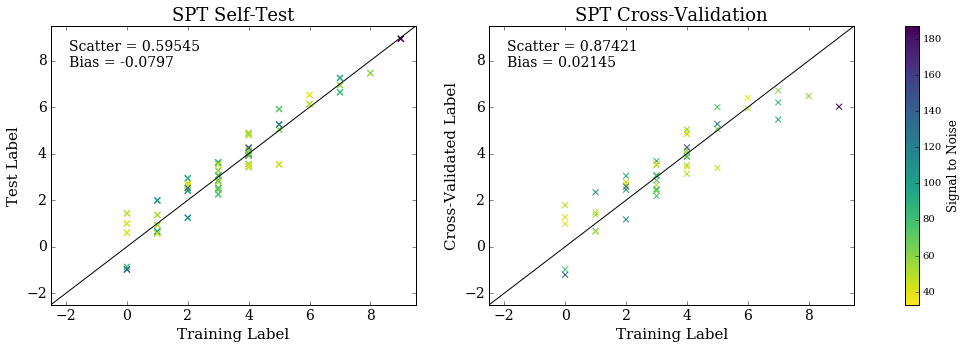
\includegraphics[width=18cm]{figures/self_and_validation_test_spt_snr.png}
\end{center}
\caption{Consistency test for the West-trained spectral type model; self-test \textit{(left)}, and leave-one-out cross validation \textit{(right)}.} \label{fig:west_validation}
\end{figure}

\begin{figure}[ht]
\begin{center}
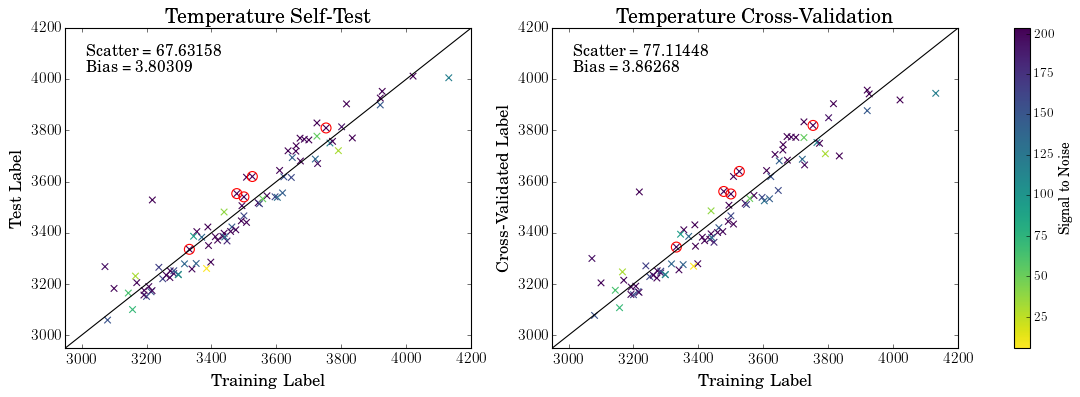
\includegraphics[width=18cm]{figures/self_and_validation_test_teff_snr.png}
\includegraphics[width=18cm]{figures/self_and_validation_test_fe_h_snr.png}
\end{center}
\caption{Consistency test for the Mann-trained temperature/metallicity type model; self-test \textit{(left)}, and leave-one-out cross validation \textit{(right)}.} \label{fig:mann_validation}
\end{figure}

%---------------------------
\begin{figure}[ht]
\plotone{figures/Spectral_Sequence_1.pdf}
\plotone{figures/Spectral_Sequence_2.pdf}
\plotone{figures/Spectral_Sequence_3.pdf}
\caption{ Spectral sequence of dwarfs in training set M0-M9; separate plots show three detector chips of APOGEE spectrum (black), the best fit Cannon trained model (red) with highlighted spectral type sensitive regions identified in \citealt{Desphande:2013}.} \label{fig:sp_sequence}
\end{figure}

%---------------------------
\begin{figure}[ht]
\begin{center}
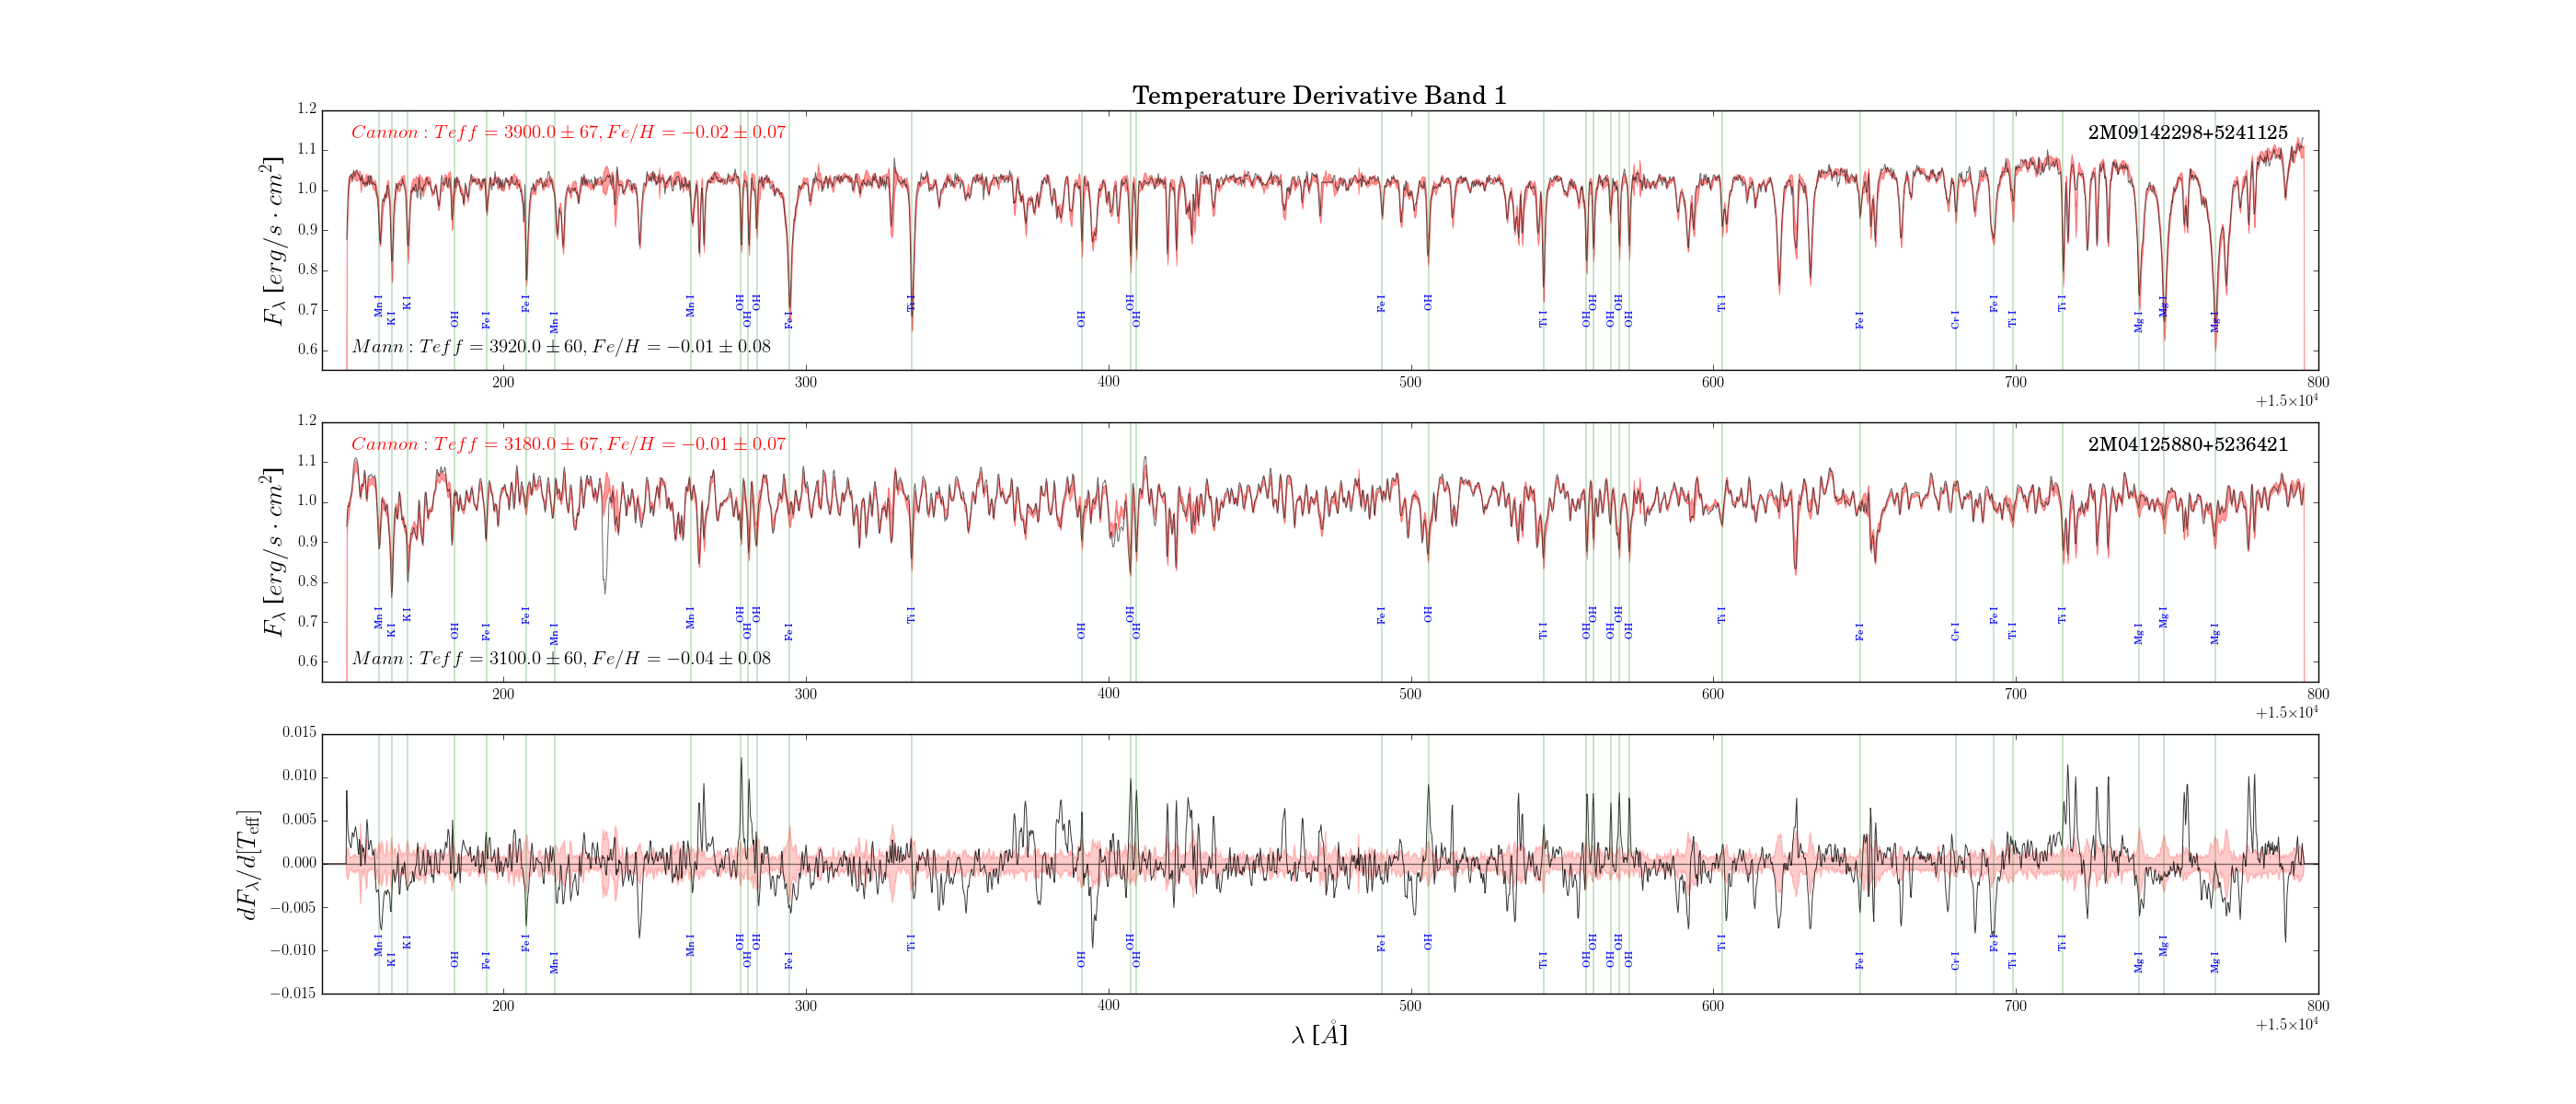
\includegraphics[width=16cm]{figures/demo_derivatives_teff1.png}
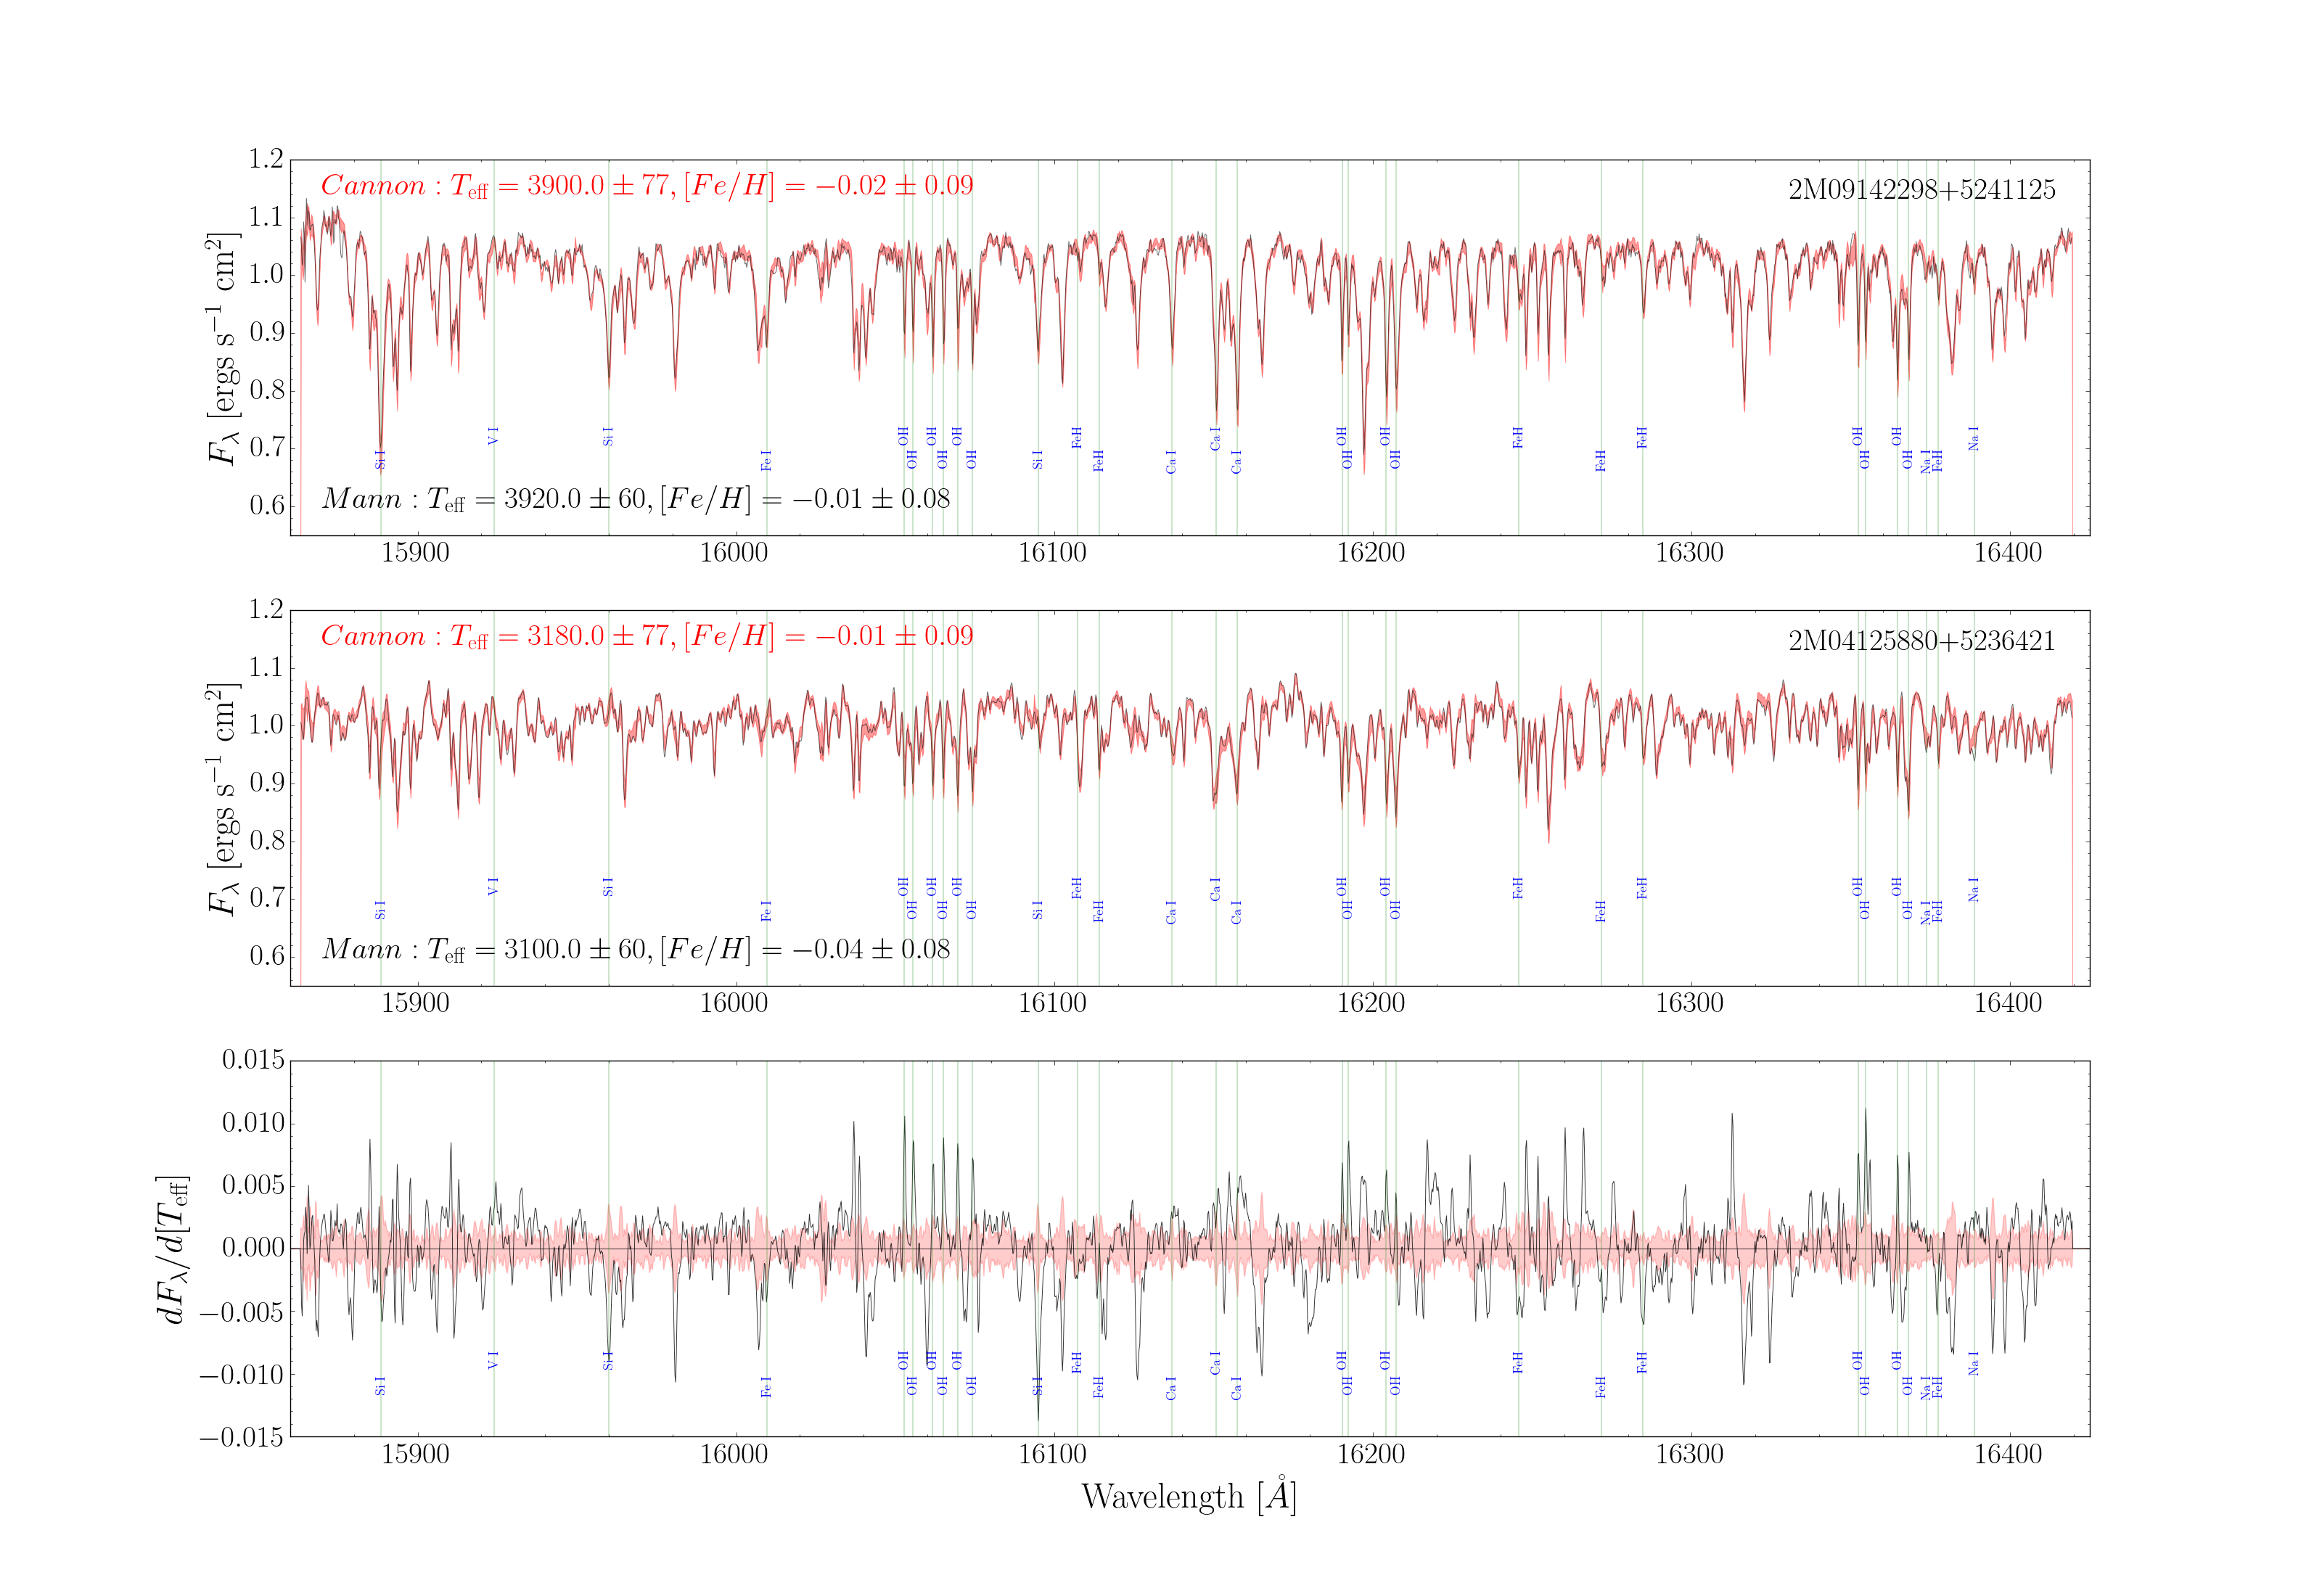
\includegraphics[width=16cm]{figures/demo_derivatives_teff2.png}
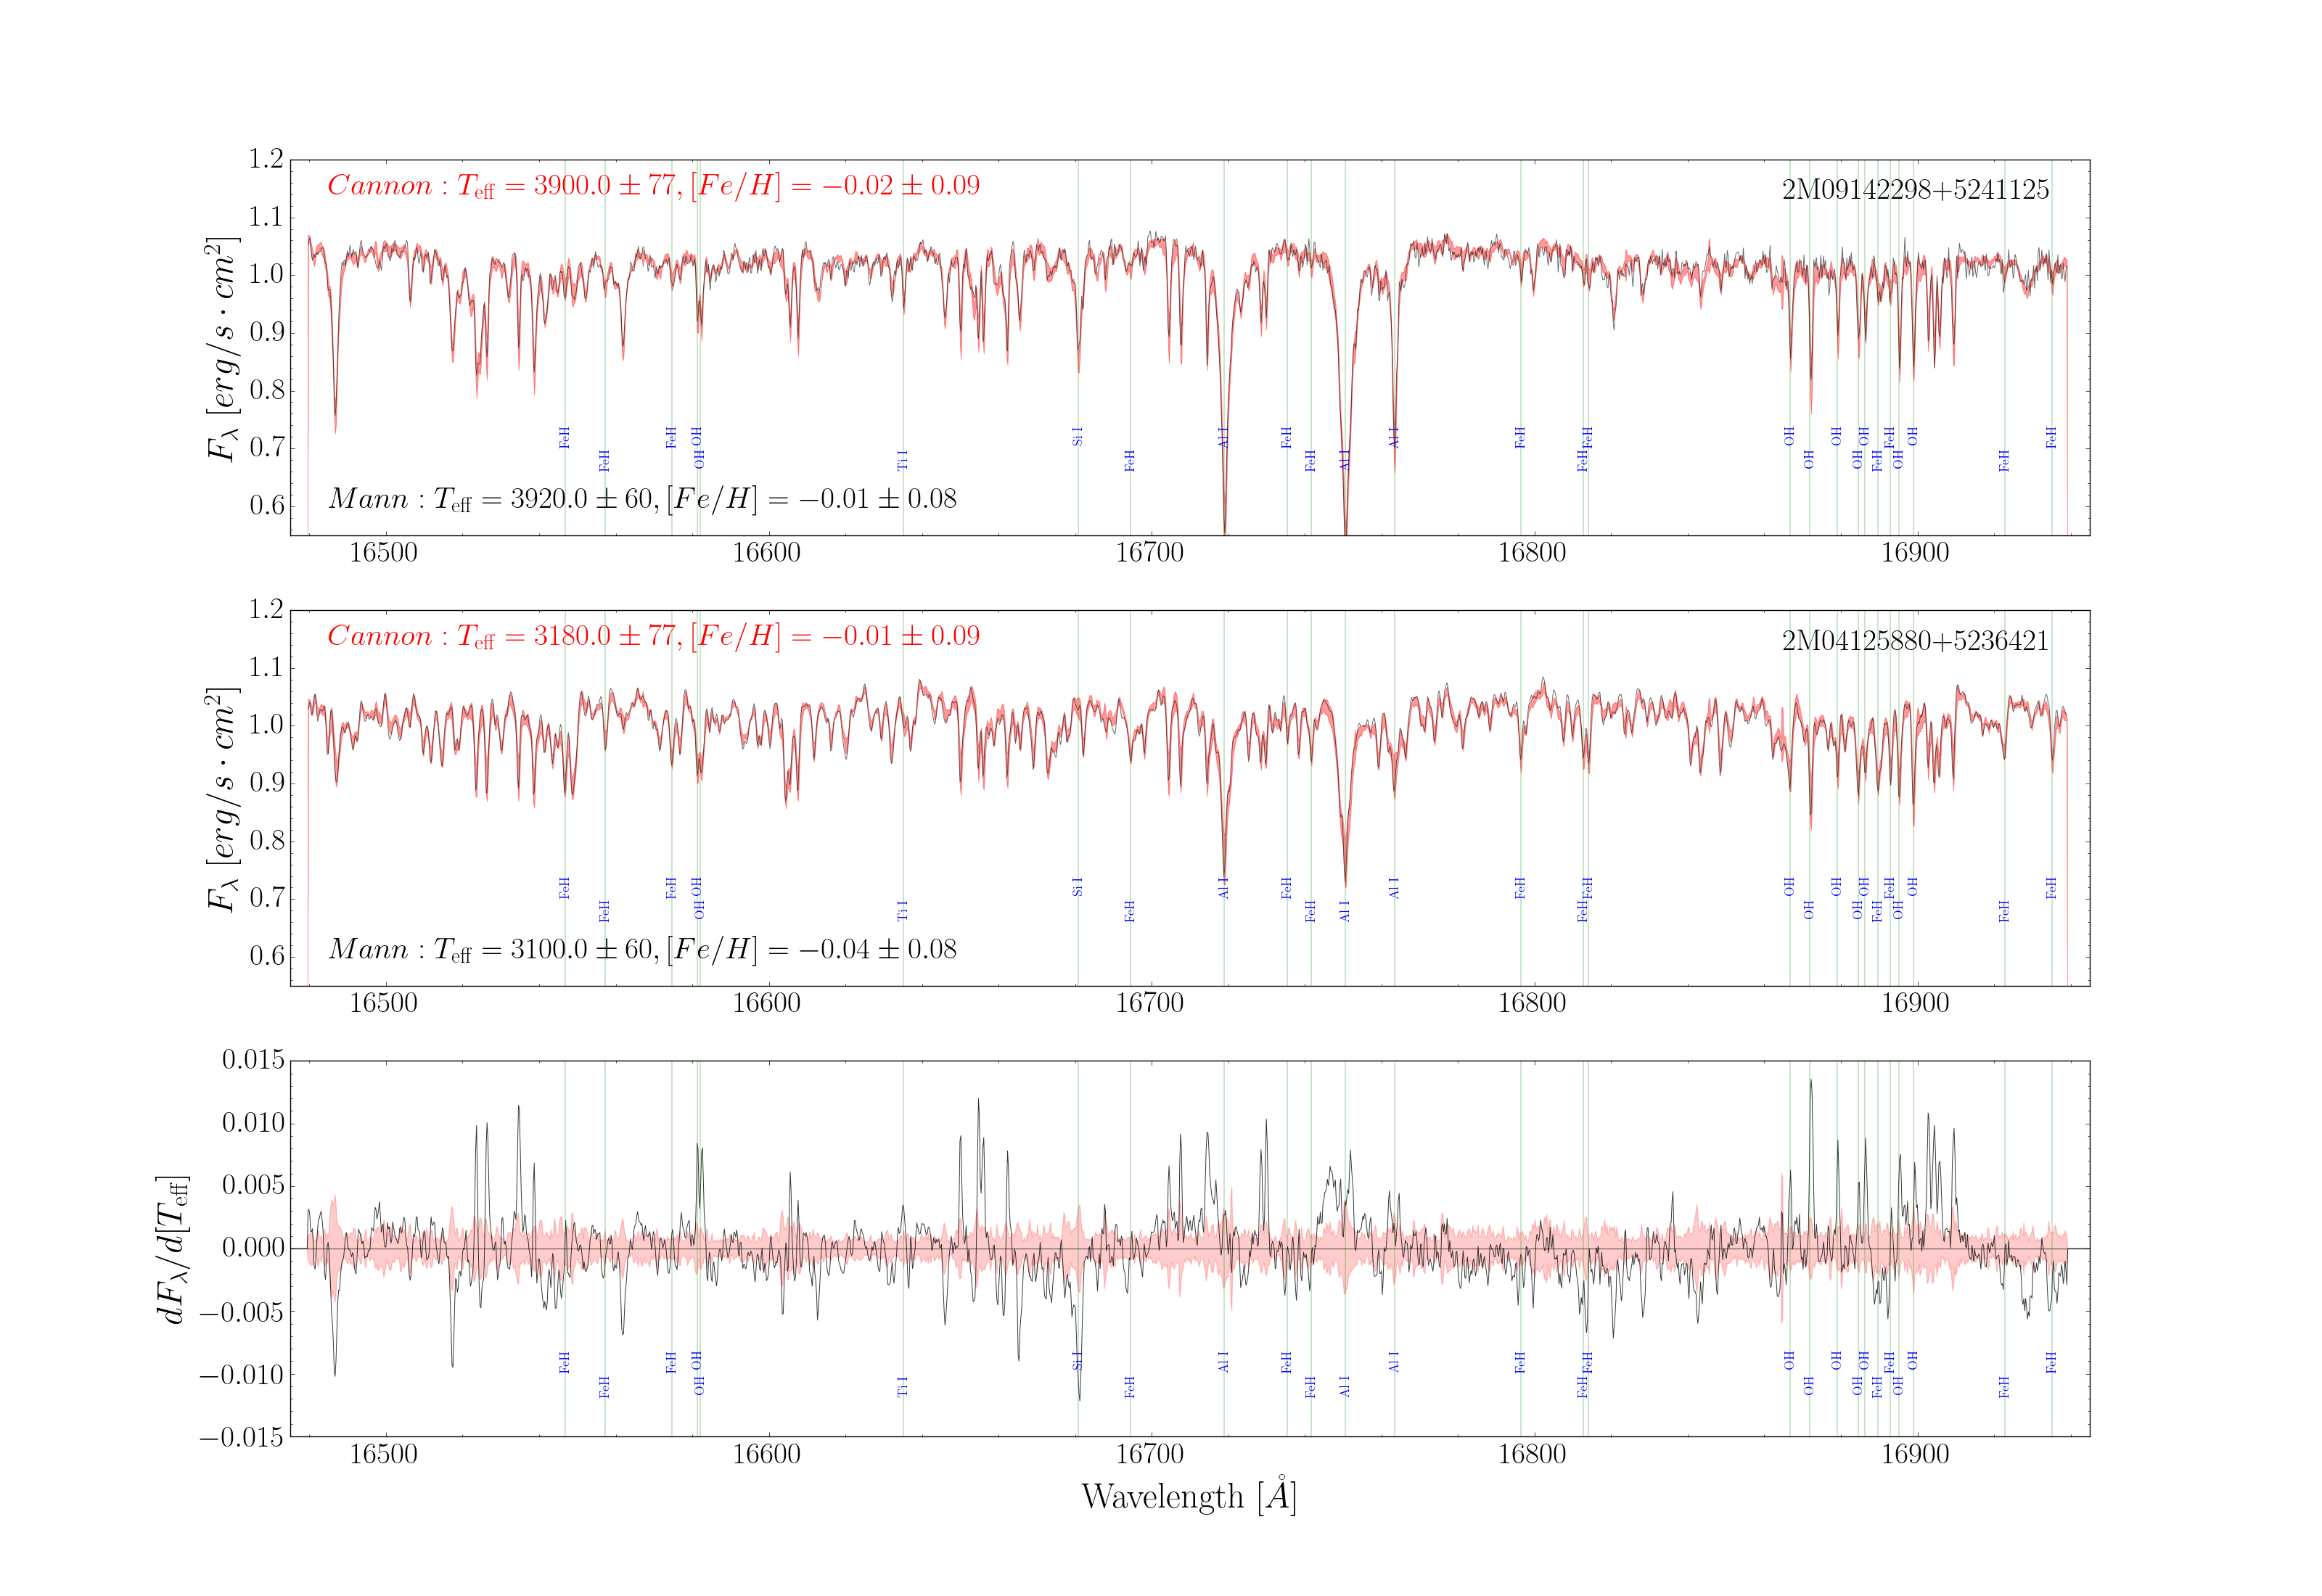
\includegraphics[width=16cm]{figures/demo_derivatives_teff3.png}
\end{center}
\caption{\textit{Top two panels of each plot:} Mann-trained model for varying temperatures, and similar metallcities. \textit{Third panel:} Derivative of the Cannon model with respect to temperature, taken at the median training temperature, T$_{\rm eff}=3463 K$}. \label{fig:demo_teff}
\end{figure}

%---------------------------
\begin{figure}[ht]
\begin{center}
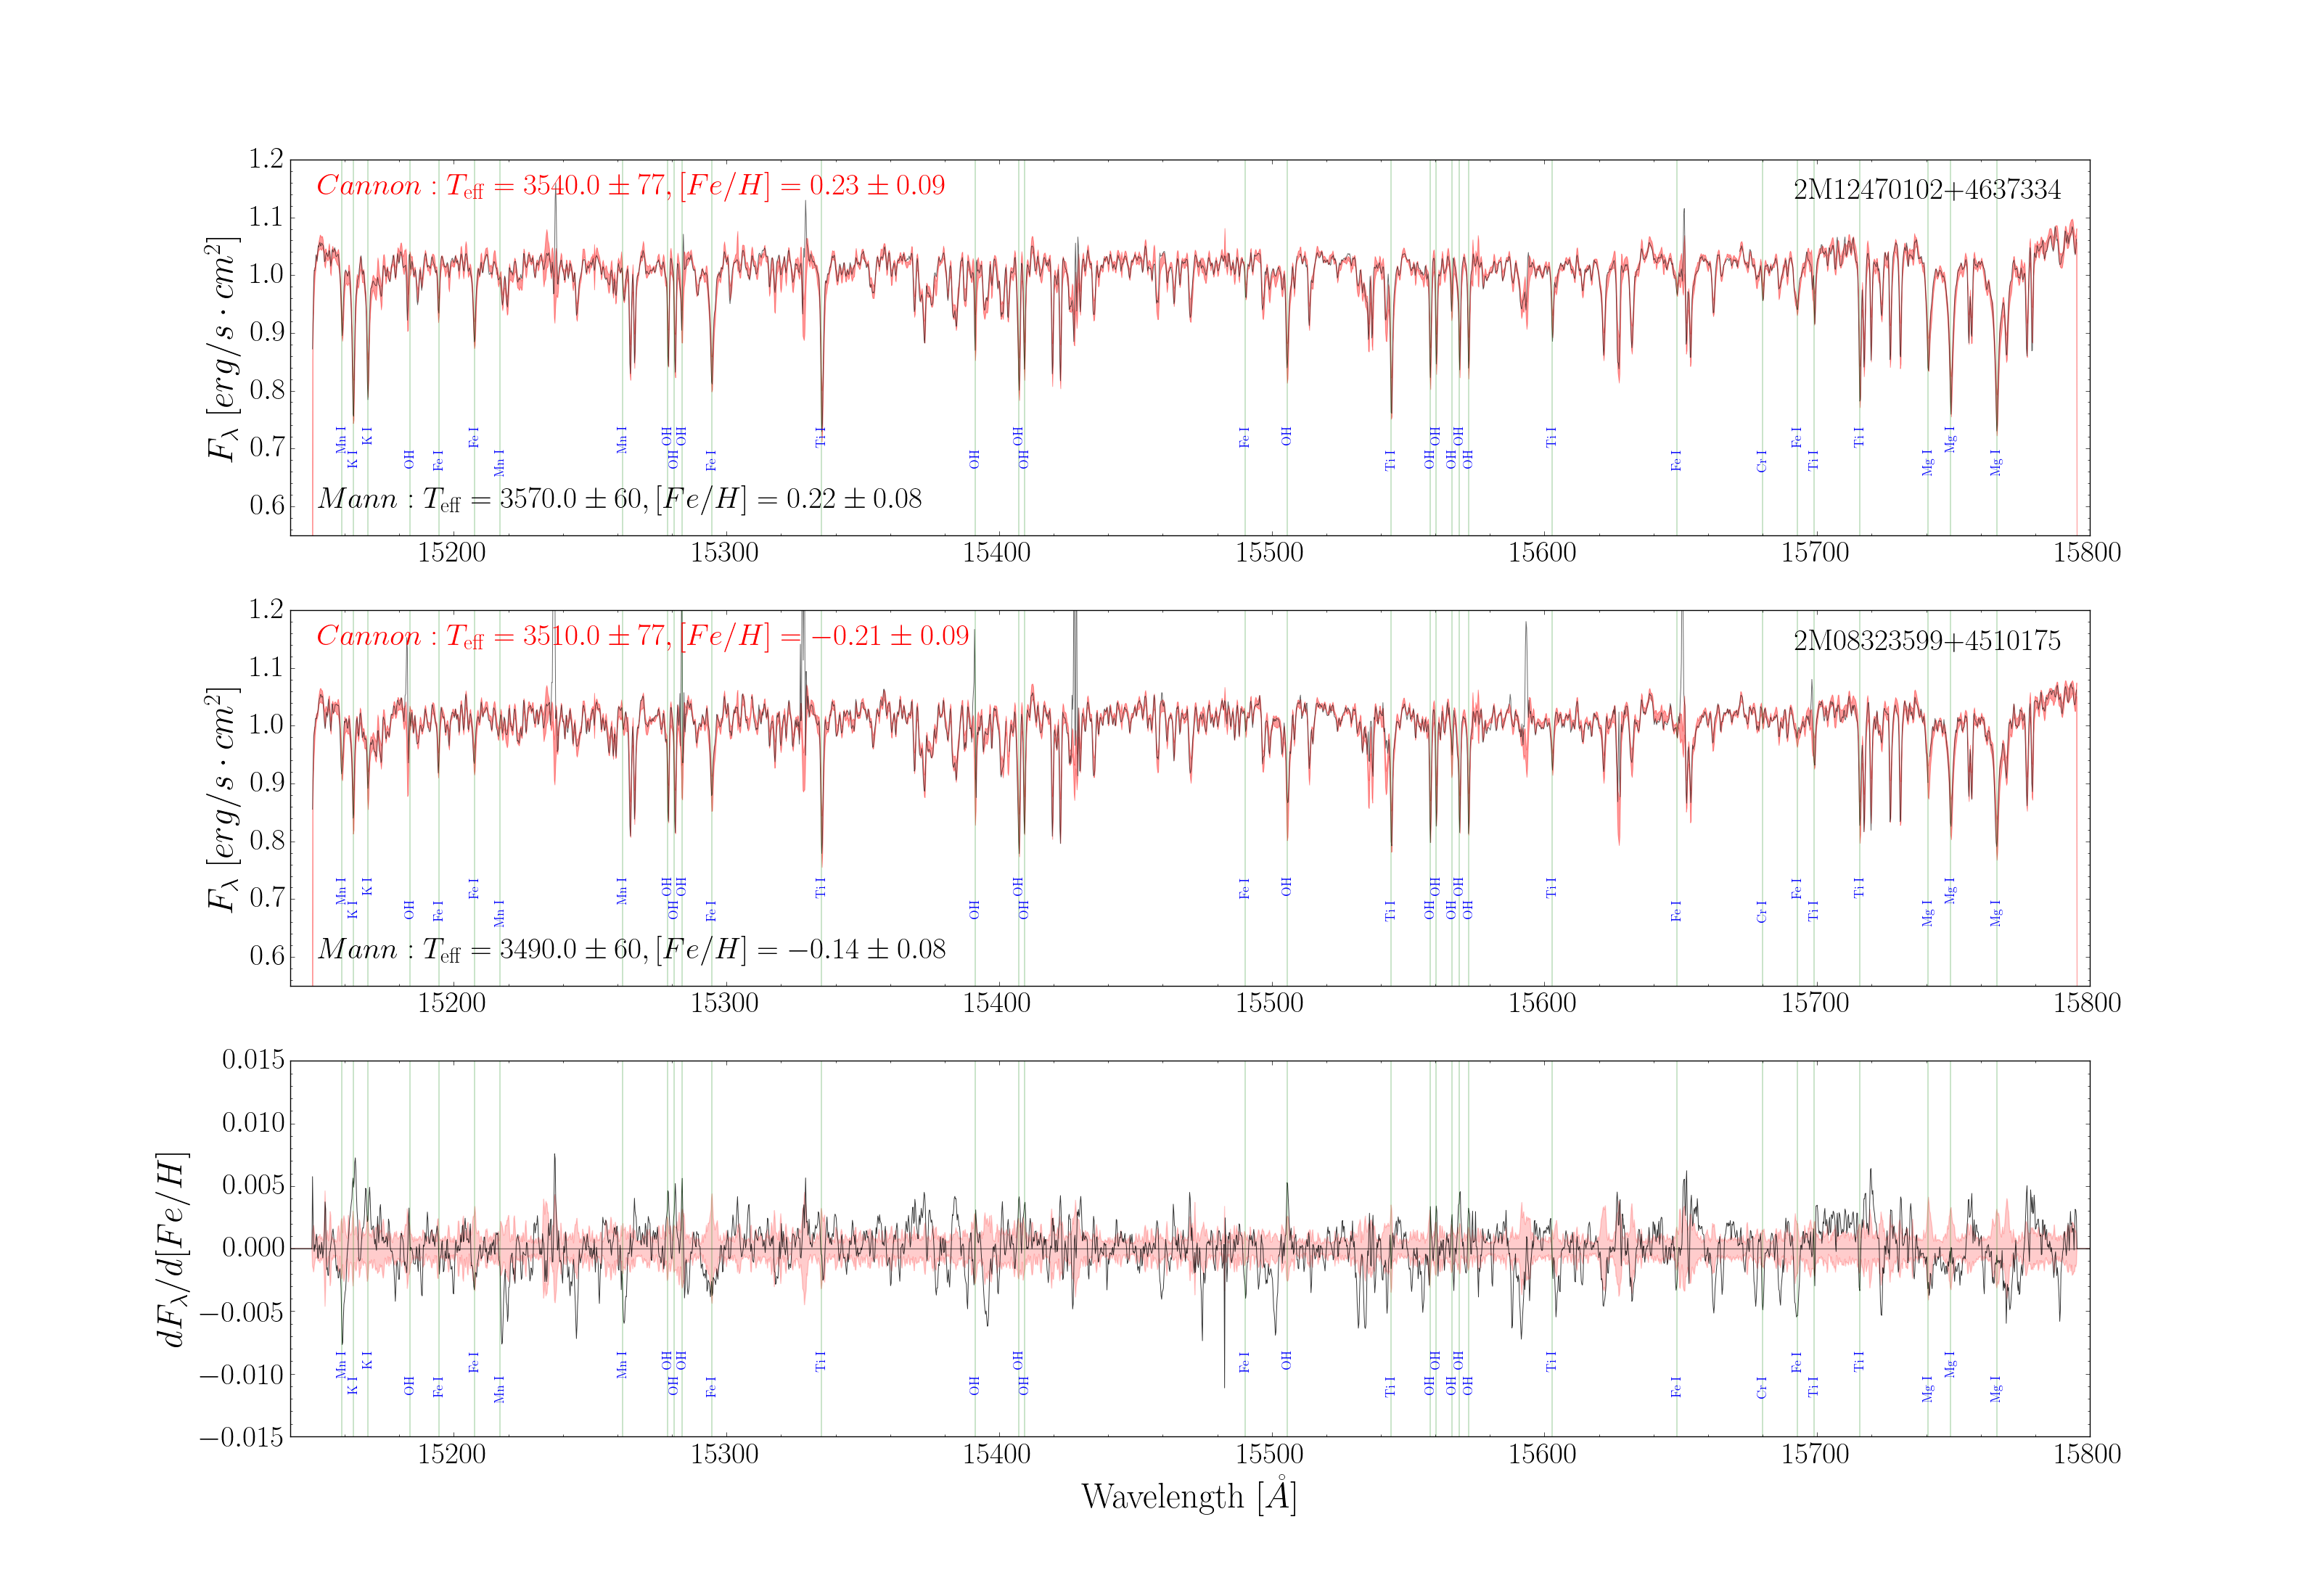
\includegraphics[width=16cm]{figures/demo_derivatives_feh1.png}
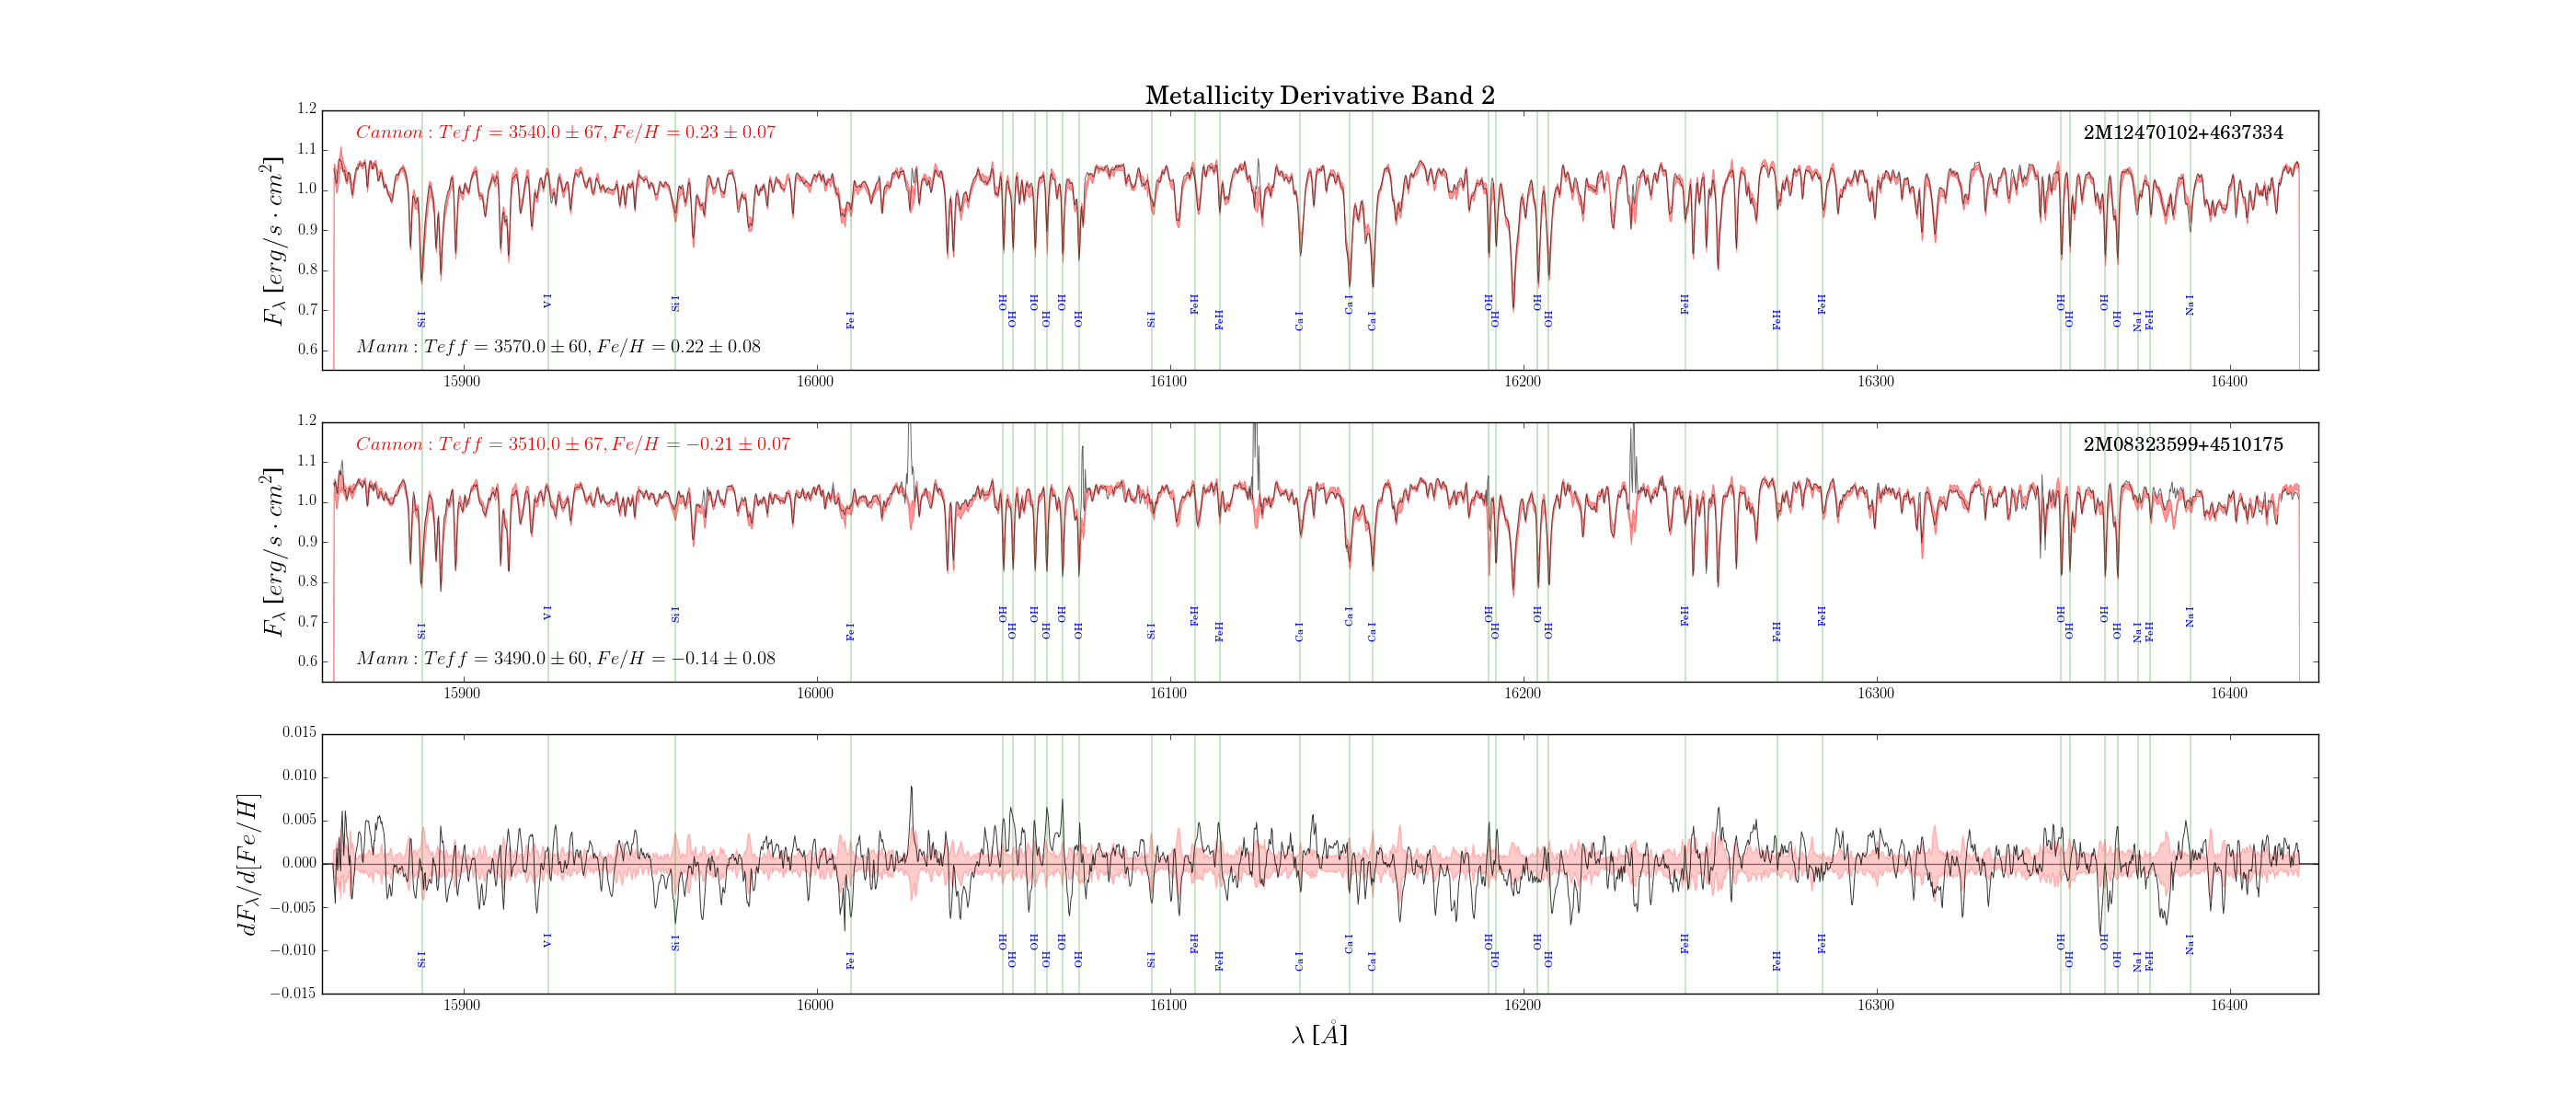
\includegraphics[width=16cm]{figures/demo_derivatives_feh2.png}
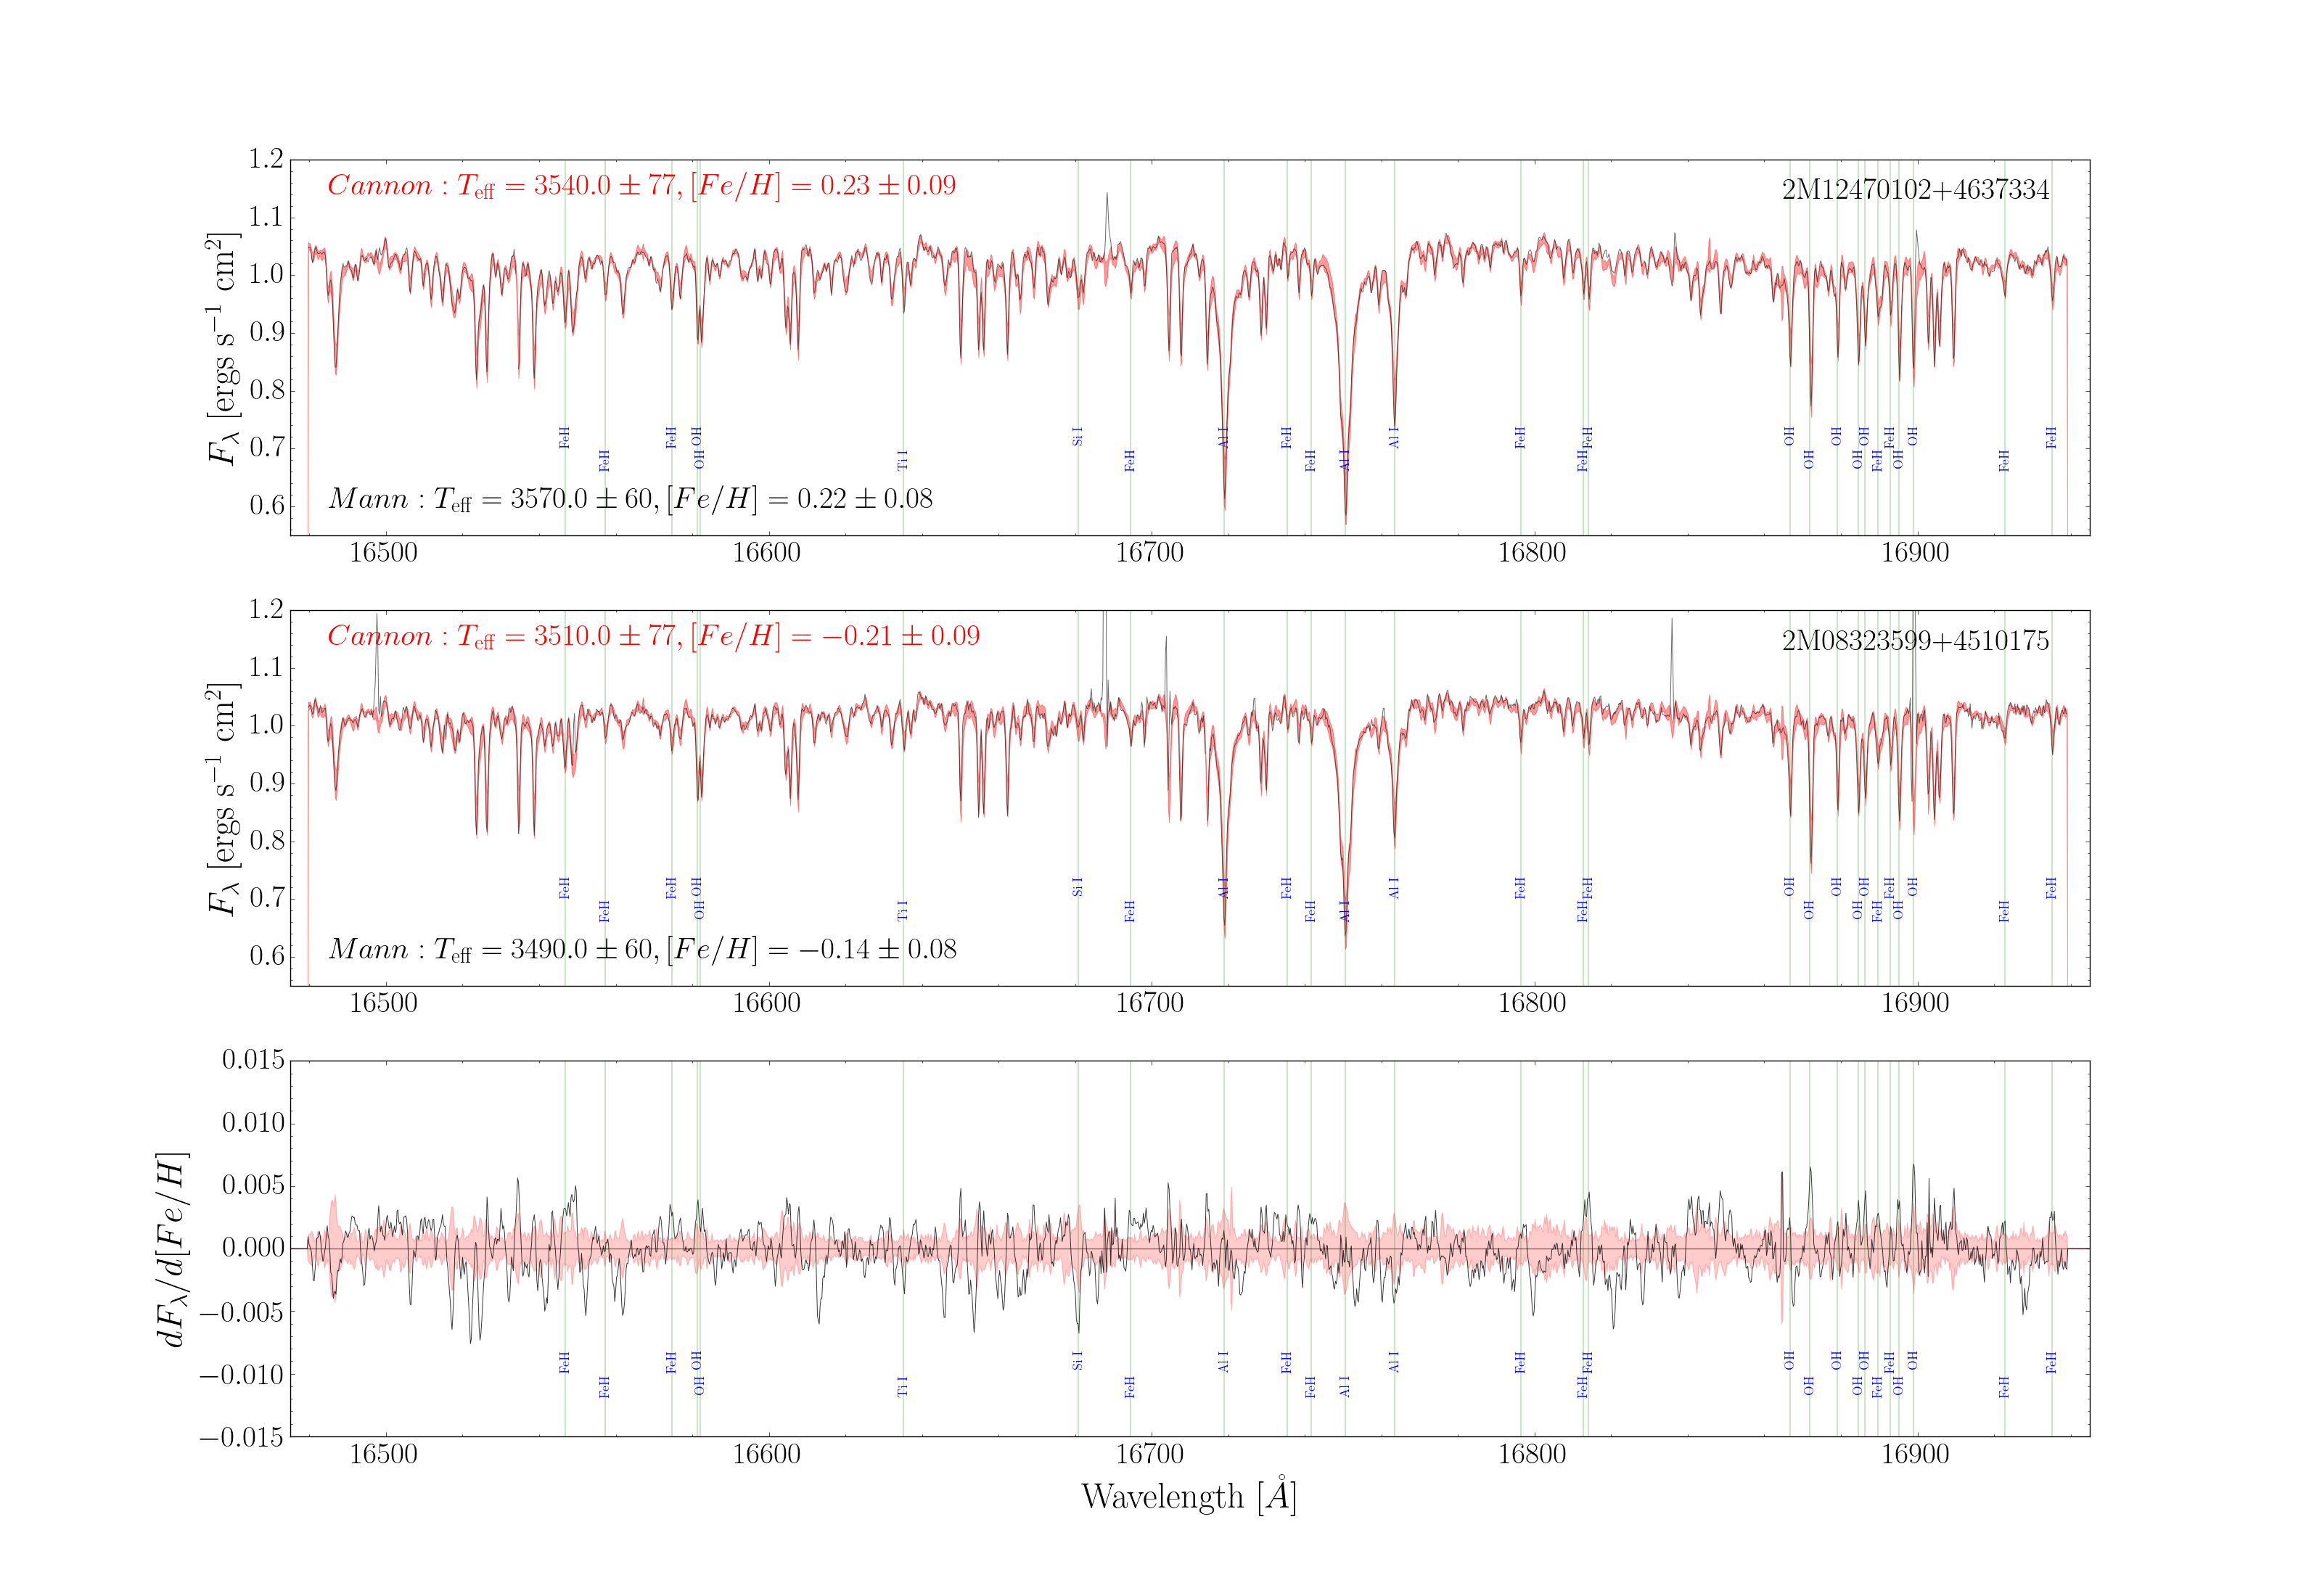
\includegraphics[width=16cm]{figures/demo_derivatives_feh3.png}
\end{center}
\caption{\textit{Top two panels of each plot:} Mann-trained model for varying metallicities and similar temperatures. \textit{Third panel:} Derivative of the Cannon model with respect to metallicity, taken at the median training metallicity, [Fe/H]$=-0.03$.} \label{fig:demo_feh}
\end{figure}

%---------------------------
\begin{figure}[ht]
\begin{center}
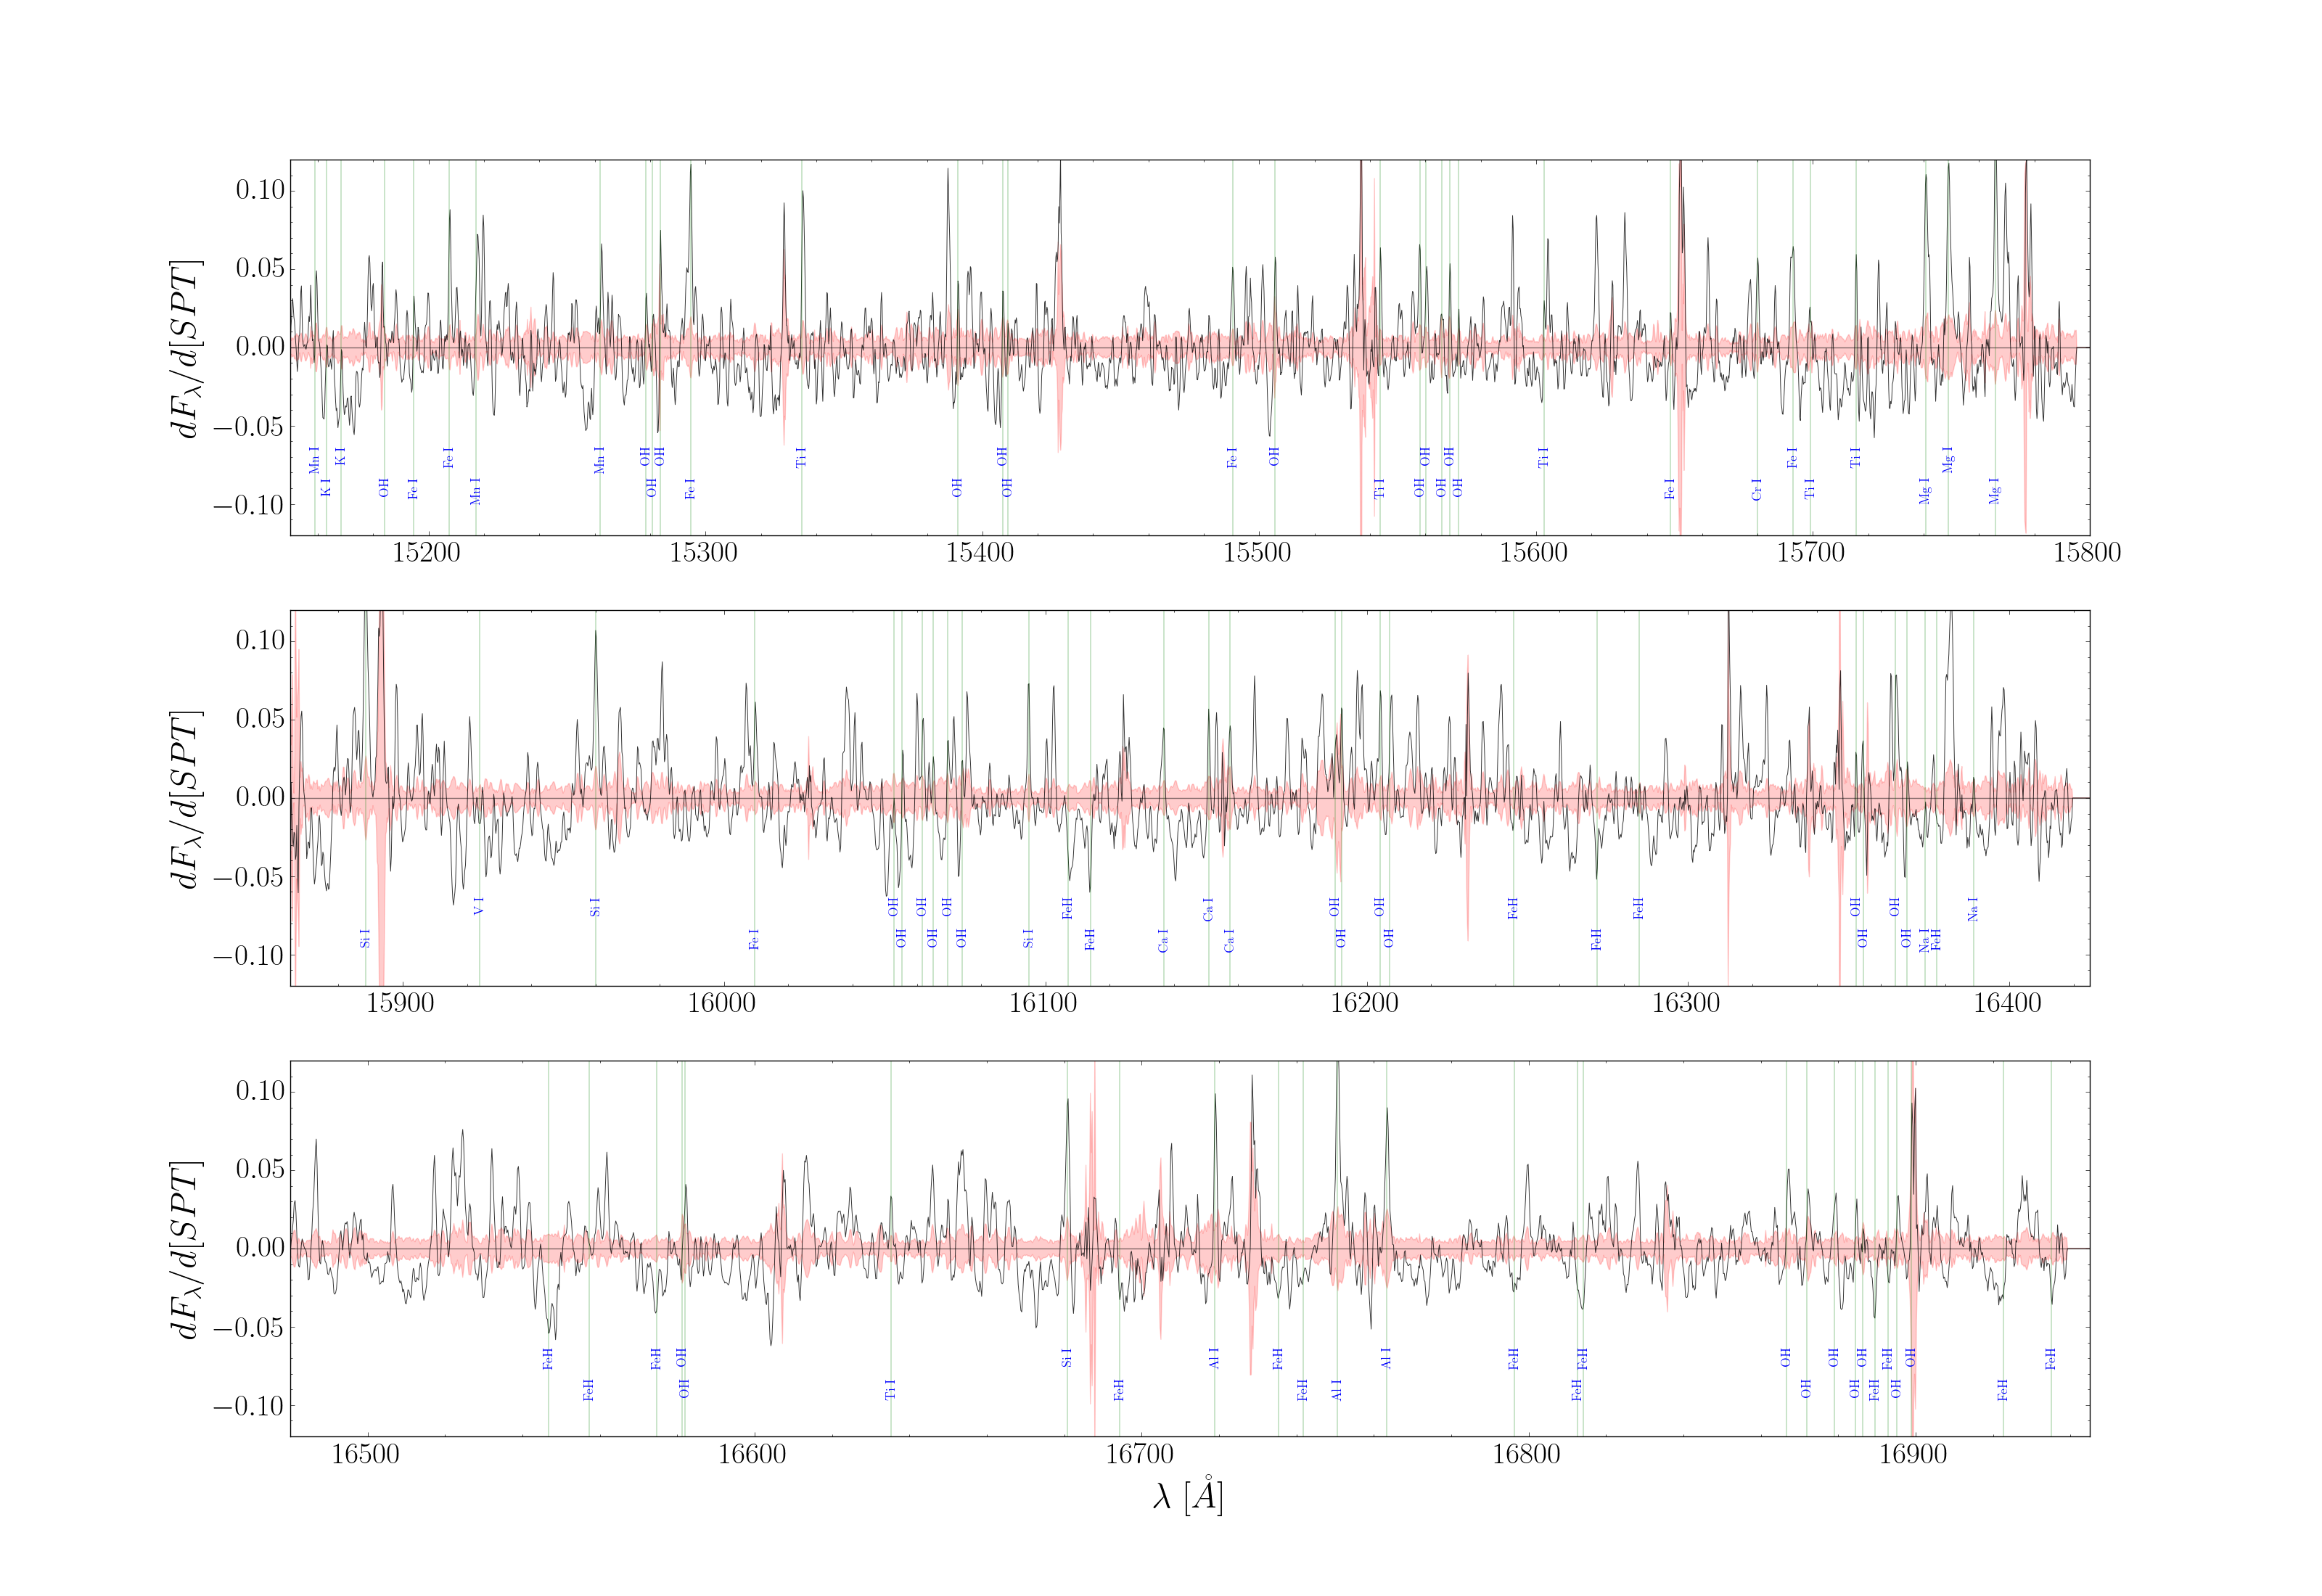
\includegraphics[width=16cm]{figures/derivative_jackknife_spt.png}
\end{center}
\caption{Derivative plots for spectral type model taken at the median training spectral type, SPT$=3$.} \label{fig:west_derivative}
\end{figure}

\begin{figure}[ht]
\begin{center}
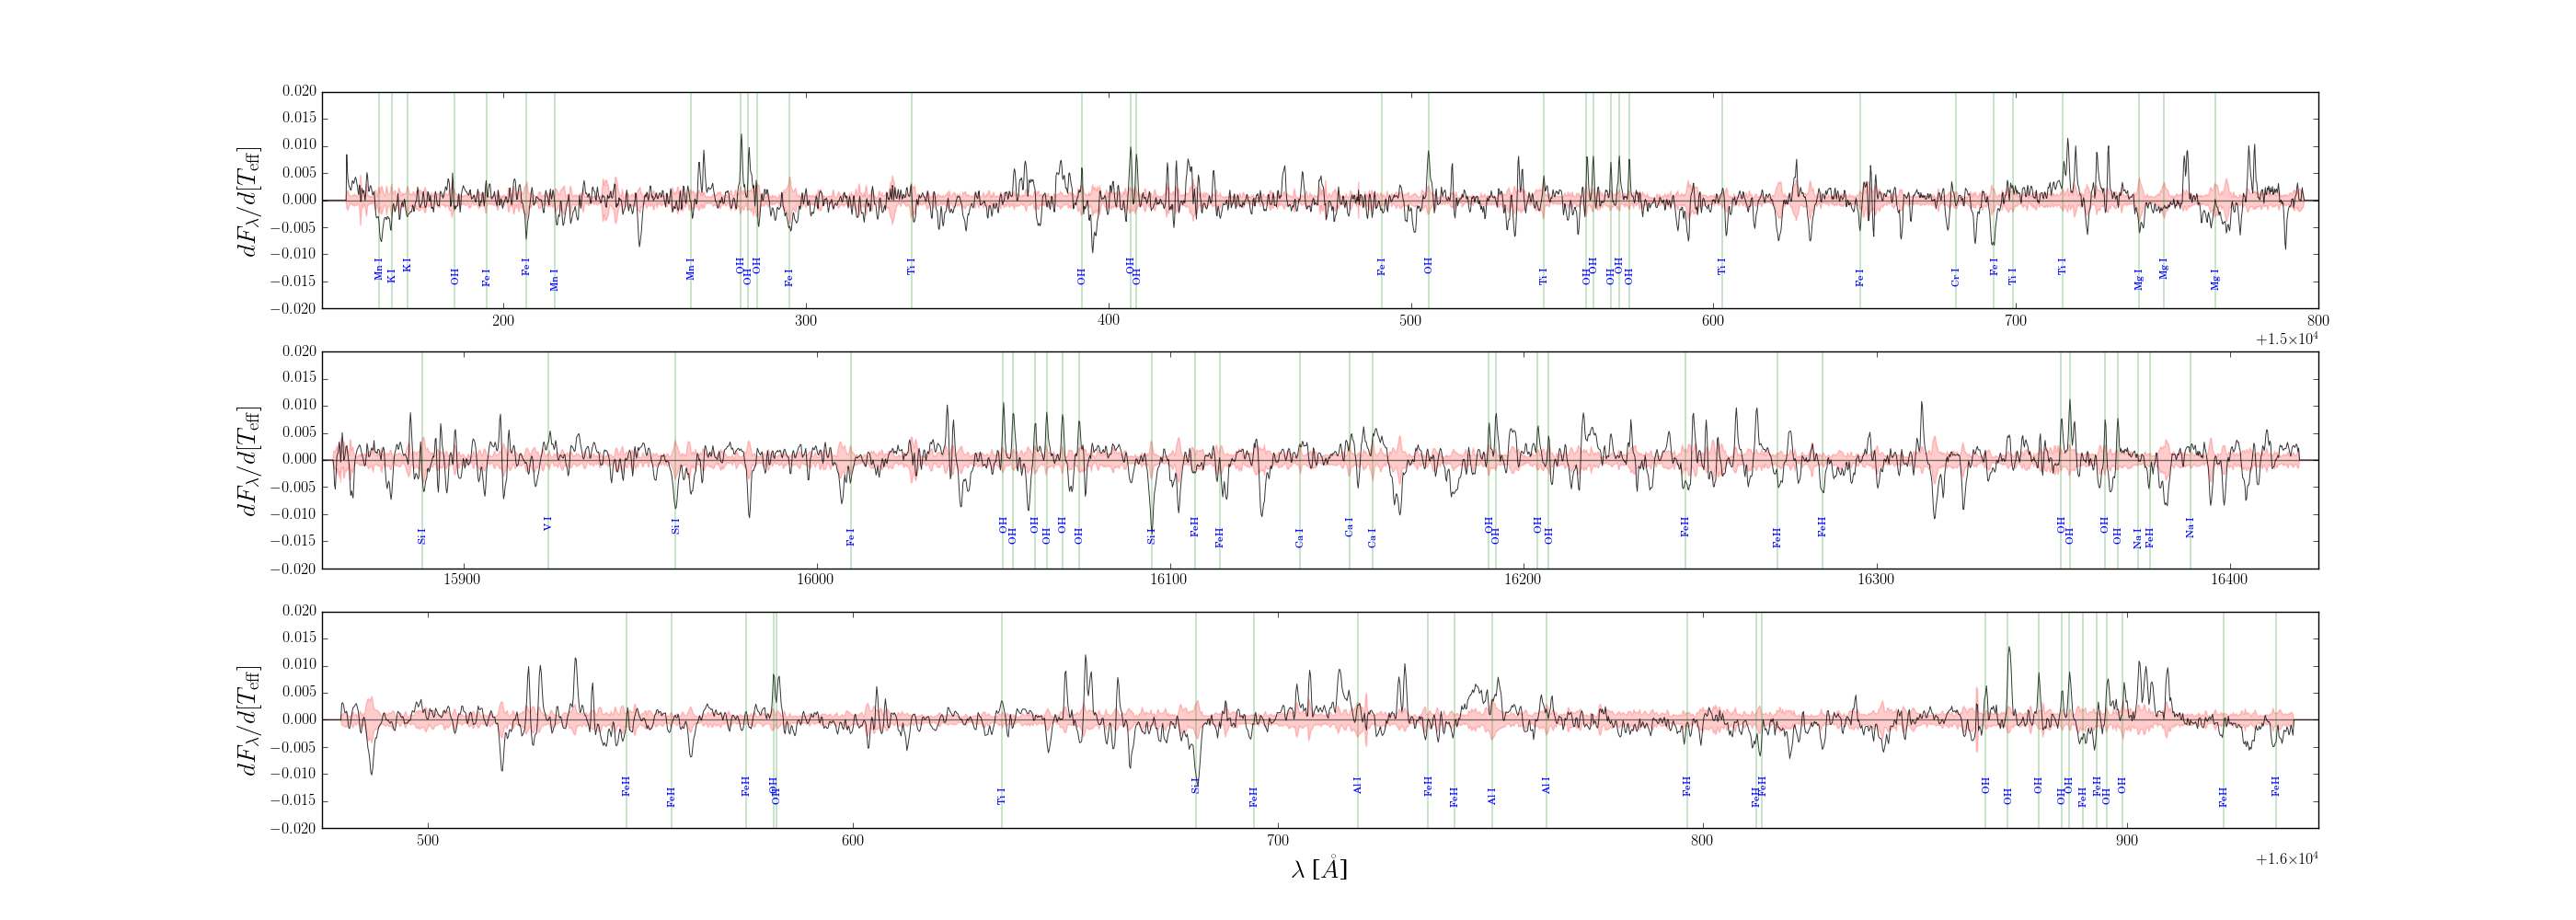
\includegraphics[width=16cm]{figures/derivative_jackknife_teff.png}
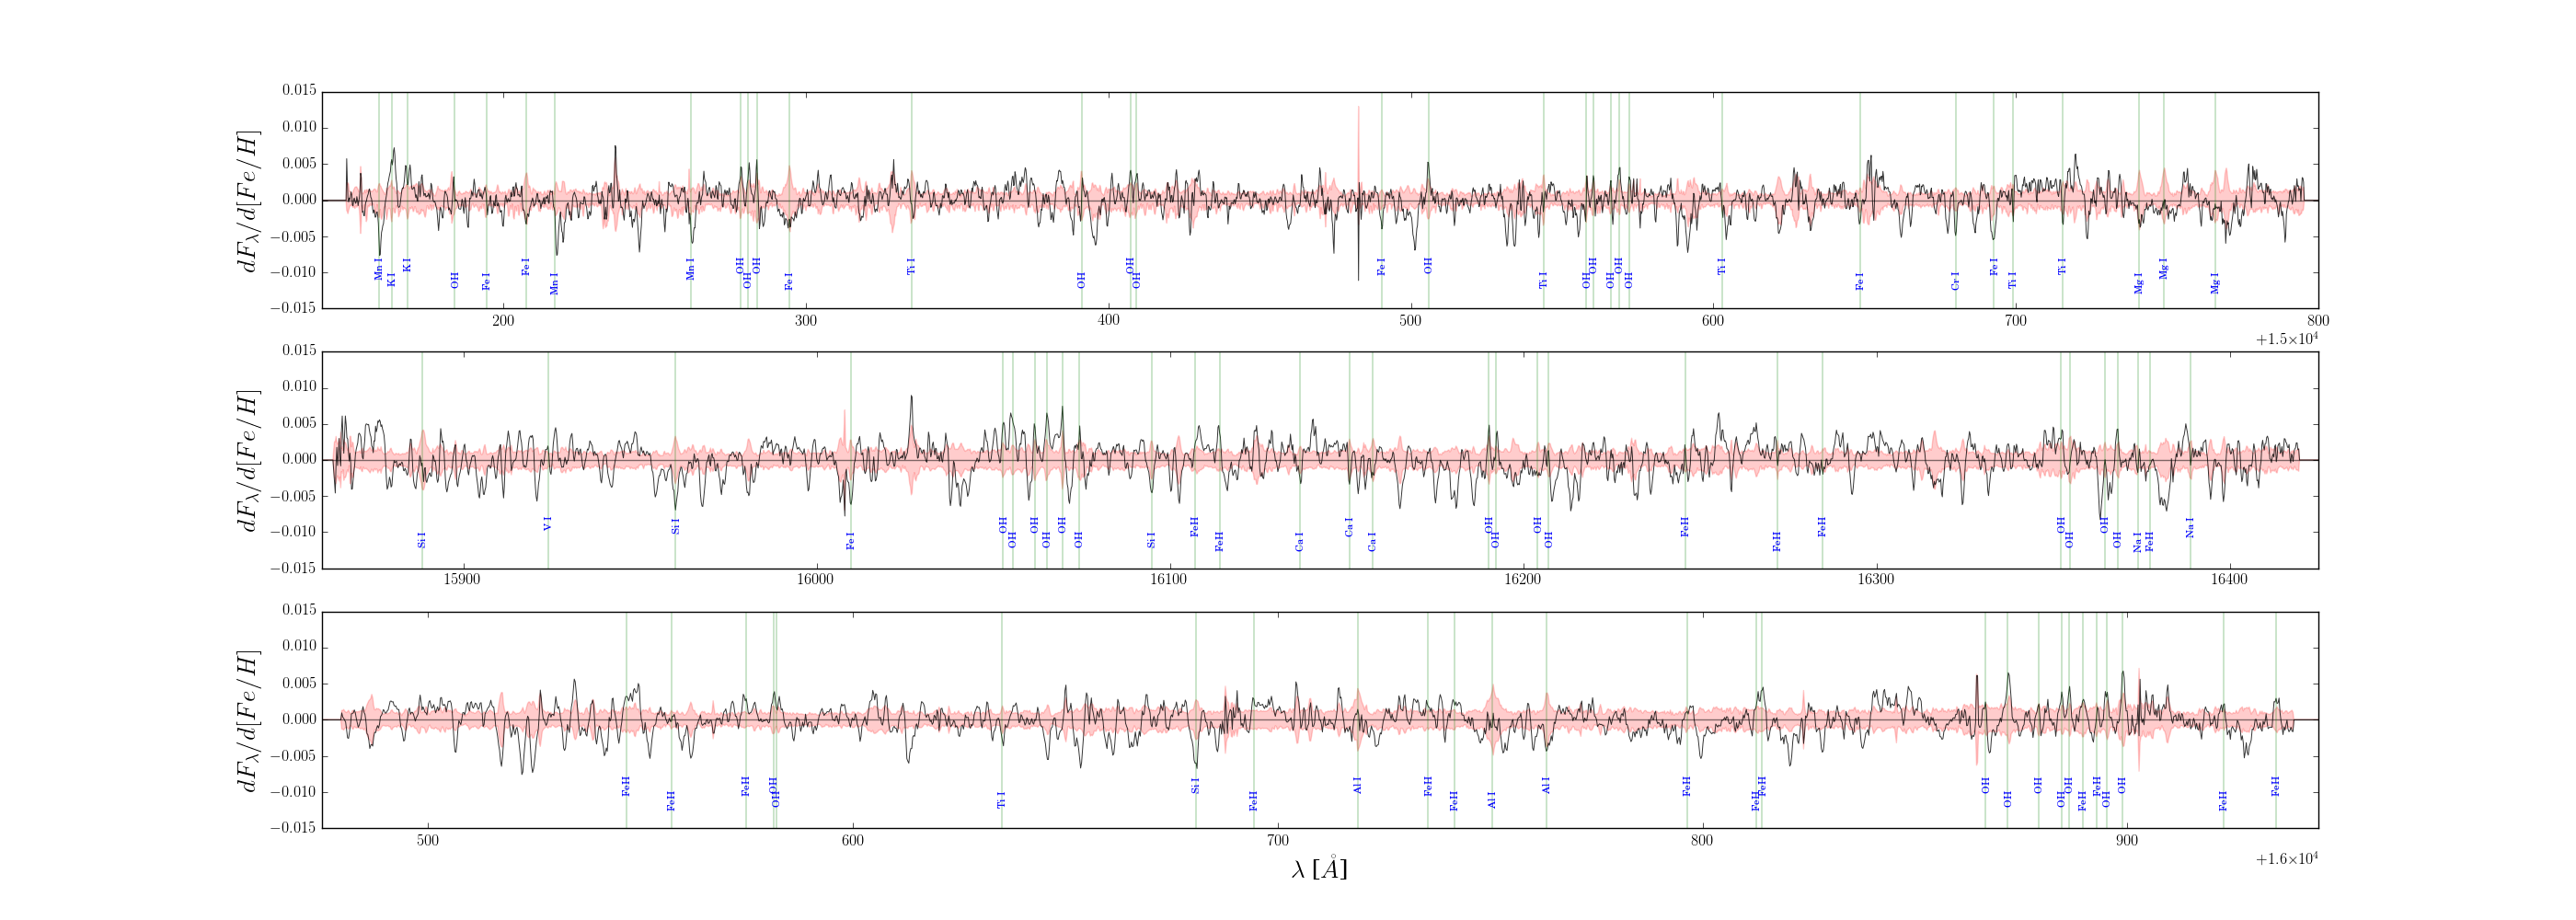
\includegraphics[width=16cm]{figures/derivative_jackknife_feh.png}
\end{center}
\caption{Derivative plots for physical parameter model. \textit{Top:} Derivative of flux with repsect to temperature taken at the median training temperature, T$_{\rm eff}=3463K$. \textit{Bottom:} Derivative of flux with repsect to metallicity taken at the median training metallicity, [Fe/H]$=-0.03$ dex.} \label{fig:mann_derivative}
\end{figure}

%---------------------------
\begin{figure}[!htb]
\minipage{0.32\textwidth}
  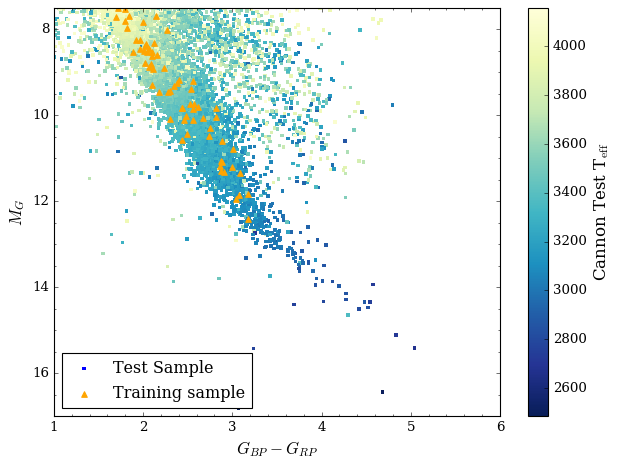
\includegraphics[width=\linewidth]{figures/test_cmd_teff.png}
\endminipage\hfill
\minipage{0.32\textwidth}
  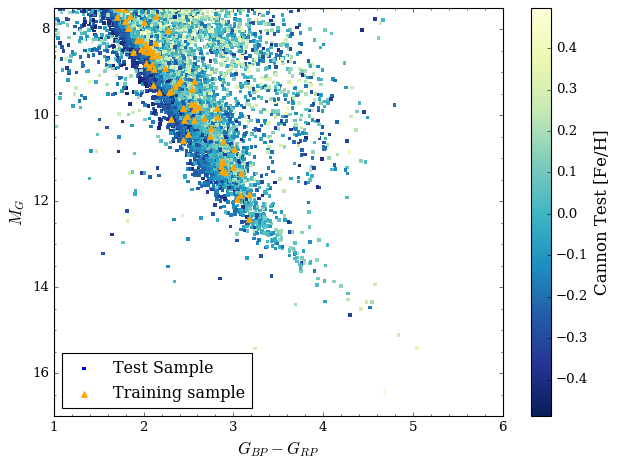
\includegraphics[width=\linewidth]{figures/test_cmd_feh.png}
\endminipage\hfill
\minipage{0.32\textwidth}%
  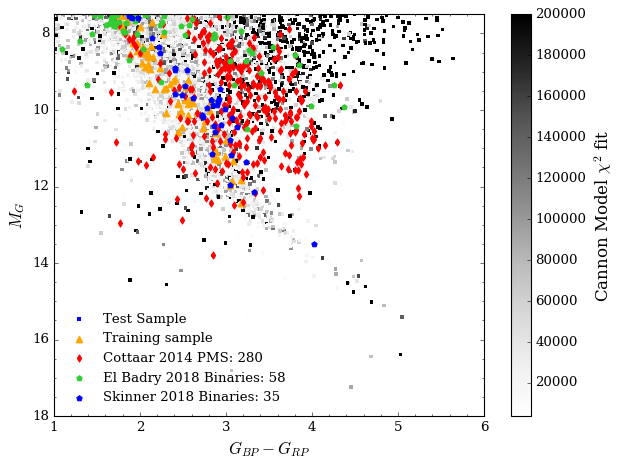
\includegraphics[width=\linewidth]{figures/test_cmd_chisq.png}
\endminipage
\end{figure}

%%==========================================================================================
%% Tables

\newpage 

% \startlongtable
% \begin{deluxetable*}{ccc|ccc|ccc}
% \tablecaption{Cannon results for Temperature/Metallicity model \label{mann_results}}
% \tabletypesize{\scriptsize}
% \tablehead{
% \multicolumn{3}{c}{\underline{Designation}} & \multicolumn{3}{c}{\underline{Temperature (K)}} & \multicolumn{3}{c}{\underline{Metallicity (dex)}} \\
% 	  \colhead{2MASS ID} & \colhead{RA}   & \colhead{DEC}
%     & \colhead{Training} & \colhead{Test} & \colhead{LOOCV}
%     & \colhead{Training} & \colhead{Test} & \colhead{LOOCV}  
% } 
% \startdata
% 2M00182256+4401222 & 4.59542   & 44.02278  & 3603        & 3532       & 3519        & -0.3       & -0.27     & -0.24      \\
% 2M00182549+4401376 & 4.60779   & 44.02734  & 3218        & 3527       & 3554        & -0.3       & -0.28     & -0.27      \\
% 2M00285391+5022330 & 7.22488   & 50.37588  & 3207        & 3185       & 3188        & 0.11       & 0.05      & 0.02       \\
% 2M00401001+0308050 & 10.04169  & 3.13473   & 3725        & 3783       & 3778        & 0.04       & 0.11      & 0.13       \\
% 2M00580115+3919111 & 14.50482  & 39.31977  & 3157        & 3094       & 3101        & -0.07      & -0.01     & 0.03       \\
% 2M01232542+1638384 & 20.8559   & 16.64401  & 3272        & 3218       & 3217        & 0.1        & 0.03      & 0.0        \\
% 2M02001278+1303112 & 30.05402  & 13.05196  & 3080        & 3057       & 3074        & -0.16      & -0.1      & -0.01      \\
% 2M02361535+0652191 & 39.06358  & 6.87167   & 3284        & 3249       & 3253        & -0.12      & -0.29     & -0.29      \\
% 2M03044335+6144097 & 46.18104  & 61.73583  & 3500        & 3468       & 3467        & -0.12      & -0.26     & -0.27      \\
% 2M03553688+5214291 & 58.90373  & 52.2414   & 3435        & 3381       & 3369        & -0.35      & -0.25     & -0.18      \\
% 2M04125880+5236421 & 63.24499  & 52.61165  & 3100        & 3181       & 3200        & -0.04      & -0.01     & 0.01       \\
% 2M04310001+3647548 & 67.75003  & 36.79855  & 3419        & 3371       & 3369        & 0.08       & 0.11      & 0.1        \\
% 2M05030563+2122362 & 75.77354  & 21.37664  & 3155        & 3290       & 3503        & 0.06       & -0.15     & -0.36      \\
% 2M05222053+3031097 & 80.58561  & 30.51933  & 3389        & 3417       & 3426        & 0.28       & 0.2       & 0.14       \\
% 2M05312734-0340356 & 82.86417  & -3.67722  & 3801        & 3820       & 3854        & 0.49       & 0.49      & 0.37       \\
% 2M05413073+5329239 & 85.37804  & 53.48987  & 3765        & 3752       & 3755        & 0.19       & 0.15      & 0.13       \\
% 2M05420897+1229252 & 85.53833  & 12.48956  & 3250        & 3226       & 3235        & -0.22      & -0.34     & -0.31      \\
% 2M06000351+0242236 & 90.01458  & 2.70657   & 3214        & 3164       & 3165        & 0.07       & 0.05      & 0.03       \\
% 2M06011106+5935508 & 90.2961   & 59.59713  & 3340        & 3258       & 3255        & -0.09      & -0.05     & -0.03      \\
% 2M06112610+1032599 & 92.8588   & 10.54998  & 3636        & 3711       & 3698        & -0.39      & -0.42     & -0.39      \\
% 2M06544902+3316058 & 103.70411 & 33.26823  & 3448        & 3364       & 3359        & -0.02      & 0.04      & 0.06       \\
% 2M07171706-0501031 & 109.32108 & -5.01754  & 3193        & 3159       & 3168        & -0.09      & -0.12     & -0.09      \\
% 2M07272450+0513329 & 111.852   & 5.2263    & 3317        & 3285       & 3285        & -0.11      & -0.2      & -0.19      \\
% 2M07444018+0333089 & 116.16744 & 3.55252   & 3217        & 3176       & 3174        & 0.23       & 0.26      & 0.15       \\
% 2M08031949+5250387 & 120.83131 & 52.84402  & 3508        & 3622       & 3626        & -0.26      & -0.24     & -0.24      \\
% 2M08083284+5304377 & 122.13679 & 53.07712  & 3398        & 3280       & 3273        & 0.0        & 0.08      & 0.09       \\
% 2M08103429-1348514 & 122.64277 & -13.81427 & 3544        & 3517       & 3515        & 0.0        & 0.0       & 0.0        \\
% 2M08155393+3136392 & 123.97459 & 31.61077  & 3753        & 3810       & 3821        & 0.16       & 0.07      & 0.03       \\
% 2M08323599+4510175 & 128.14998 & 45.17153  & 3494        & 3505       & 3506        & -0.14      & -0.21     & -0.21      \\
% 2M08370799+1507475 & 129.28319 & 15.12944  & 3596        & 3553       & 3552        & -0.17      & -0.26     & -0.27      \\
% 2M08524084+2818589 & 133.17018 & 28.31634  & 3166        & 3213       & 3239        & 0.31       & 0.5       & 0.27       \\
% 2M08585633+0828259 & 134.73479 & 8.47384   & 3200        & 3142       & 3147        & -0.04      & -0.09     & -0.08      \\
% 2M09142298+5241125 & 138.595   & 52.68639  & 3920        & 3900       & 3879        & -0.01      & -0.02     & 0.01       \\
% 2M09174473+4612246 & 139.4363  & 46.20685  & 3478        & 3548       & 3556        & 0.04       & -0.02     & -0.03      \\
% 2M09214911+4330284 & 140.45447 & 43.50784  & 3170        & 3196       & 3206        & 0.16       & 0.23      & 0.19       \\
% 2M09285333-0722148 & 142.22221 & -7.37095  & 3508        & 3445       & 3440        & -0.27      & -0.23     & -0.22      \\
% 2M10112218+4927153 & 152.84254 & 49.45431  & 4131        & 4007       & 3946        & 0.24       & 0.22      & 0.23       \\
% 2M10121768-0344441 & 153.07364 & -3.74563  & 3623        & 3619       & 3620        & 0.13       & 0.16      & 0.16       \\
% 2M10193634+1952122 & 154.90117 & 19.87002  & 3370        & 3384       & 3389        & 0.15       & 0.24      & 0.21       \\
% 2M10285555+0050275 & 157.23155 & 0.8411    & 3548        & 3517       & 3515        & -0.18      & -0.16     & -0.15      \\
% 2M10331367+3409120 & 158.30687 & 34.15333  & 3500        & 3518       & 3518        & -0.15      & -0.19     & -0.2       \\
% 2M10350859+3349499 & 158.7858  & 33.83055  & 3816        & 3906       & 3907        & -0.04      & 0.01      & 0.03       \\
% 2M10453795+1833111 & 161.4081  & 18.55306  & 3673        & 3773       & 3780        & 0.14       & 0.13      & 0.13       \\
% 2M10505201+0648292 & 162.71704 & 6.80826   & 3238        & 3258       & 3265        & 0.16       & 0.18      & 0.12       \\
% 2M10520440+1359509 & 163.01762 & 13.99756  & 3298        & 3230       & 3228        & -0.13      & -0.11     & -0.07      \\
% 2M11000432+2249592 & 165.01781 & 22.833    & 3463        & 3426       & 3423        & -0.11      & -0.1      & -0.09      \\
% 2M11032023+3558117 & 165.83423 & 35.97054  & 3563        & 3682       & 3551        & -0.38      & -0.58     & -0.39      \\
% 2M11052903+4331357 & 166.36992 & 43.52665  & 3619        & 3547       & 3525        & -0.37      & -0.34     & -0.3       \\
% 2M11054316+1014093 & 166.42966 & 10.23605  & 3439        & 3395       & 3393        & -0.03      & -0.06     & -0.07      \\
% 2M11091225-0436249 & 167.30106 & -4.60695  & 3661        & 3743       & 3748        & -0.03      & -0.09     & -0.1       \\
% 2M11263270+2145262 & 171.63622 & 21.75719  & 3610        & 3642       & 3642        & -0.18      & -0.16     & -0.15      \\
% 2M11273856+0358359 & 171.91071 & 3.97664   & 3920        & 3932       & 3963        & 0.43       & 0.44      & 0.31       \\
% 2M11474074+0015201 & 176.9198  & 0.25553   & 3261        & 3235       & 3236        & 0.1        & 0.23      & 0.22       \\
% 2M11474440+0048164 & 176.93491 & 0.80473   & 3192        & 3155       & 3157        & -0.02      & -0.06     & -0.06      \\
% 2M11530522+1855480 & 178.27184 & 18.93002  & 3773        & 3760       & 3752        & -0.14      & -0.08     & -0.06      \\
% 2M12192028+1323524 & 184.83449 & 13.39793  & 3926        & 3954       & 3945        & 0.0        & 0.13      & 0.18       \\
% 2M12274471-0315006 & 186.93625 & -3.25018  & 3355        & 3399       & 3407        & 0.19       & 0.2       & 0.17       \\
% 2M12390461+4702234 & 189.76958 & 47.03974  & 3492        & 3447       & 3445        & 0.05       & 0.06      & 0.06       \\
% 2M12470102+4637334 & 191.75412 & 46.62587  & 3571        & 3543       & 3544        & 0.22       & 0.23      & 0.22       \\
% 2M13113464+1306461 & 197.89433 & 13.11282  & 3459        & 3407       & 3402        & -0.1       & -0.03     & -0.01      \\
% 2M13160127+1415504 & 199.00528 & 14.26403  & 3686        & 3768       & 3775        & -0.06      & -0.16     & -0.17      \\
% 2M13295979+1022376 & 202.49895 & 10.37731  & 3727        & 3674       & 3669        & -0.09      & -0.13     & -0.13      \\
% 2M13345147+3746195 & 203.71442 & 37.7721   & 3273        & 3247       & 3250        & 0.14       & 0.13      & 0.08       \\
% 2M13400879+4346380 & 205.03676 & 43.77729  & 3332        & 3322       & 3325        & -0.19      & -0.18     & -0.14      \\
% 2M13454354+1453317 & 206.43251 & 14.89139  & 3649        & 3688       & 3677        & -0.31      & -0.37     & -0.36      \\
% 2M15290936+5724418 & 232.28886 & 57.41167  & 3660        & 3719       & 3723        & -0.09      & -0.14     & -0.14      \\
% 2M15594729+4403595 & 239.94707 & 44.06654  & 3526        & 3614       & 3632        & 0.05       & 0.02      & 0.01       \\
% 2M16252459+5418148 & 246.35249 & 54.30413  & 3475        & 3407       & 3400        & -0.35      & -0.25     & -0.22      \\
% 2M16541202+1154529 & 253.5502  & 11.91464  & 3834        & 3760       & 3697        & -0.48      & -0.38     & -0.29      \\
% 2M17093153+4340531 & 257.38138 & 43.68139  & 3284        & 3242       & 3242        & 0.2        & 0.25      & 0.17       \\
% 2M17362594+6820220 & 264.10803 & 68.33932  & 3439        & 3487       & 3492        & 0.05       & -0.21     & -0.23      \\
% 2M18161819+0131277 & 274.07575 & 1.5243    & 3391        & 3350       & 3347        & -0.25      & -0.19     & -0.17      \\
% 2M18244689-0620311 & 276.1954  & -6.342    & 3412        & 3386       & 3384        & 0.01       & 0.07      & 0.08       \\
% 2M18424666+5937499 & 280.69489 & 59.63015  & 3441        & 3386       & 3385        & -0.23      & -0.32     & -0.32      \\
% 2M18424688+5937374 & 280.6958  & 59.62659  & 3345        & 3391       & 3400        & -0.3       & -0.35     & -0.33      \\
% 2M18451027+0620158 & 281.29282 & 6.33774   & 3674        & 3684       & 3688        & 0.02       & 0.03      & 0.03       \\
% 2M19142541+1755081 & 288.6059  & 17.91894  & 3725        & 3830       & 3835        & -0.08      & -0.09     & -0.09      \\
% 2M19165526+0510086 & 289.23032 & 5.16909   & 3558        & 3536       & 3538        & 0.1        & 0.08      & 0.07       \\
% 2M19500252+3235012 & 297.51022 & 32.58347  & 3385        & 3214       & 3215        & -0.18      & -0.31     & -0.28      \\
% 2M19535443+4424541 & 298.47977 & 44.41508  & 2859        & 2801       & 2889        & -0.05      & 0.08      & 0.19       \\
% 2M20032651+2952000 & 300.86075 & 29.86652  & 3144        & 3164       & 3178        & 0.06       & -0.03     & -0.09      \\
% 2M20531977+6209156 & 313.33246 & 62.1545   & 3791        & 3728       & 3712        & -0.06      & 0.04      & 0.08       \\
% 2M21065473+3844265 & 316.73013 & 38.74202  & 4021        & 4004       & 3922        & -0.22      & -0.23     & -0.11      \\
% 2M22464980+4420030 & 341.70737 & 44.33405  & 3298        & 3236       & 3235        & 0.03       & 0.03      & 0.02       \\
% 2M22563497+1633130 & 344.14517 & 16.55347  & 3720        & 3689       & 3688        & 0.21       & 0.29      & 0.28       \\
% 2M23060482+6355339 & 346.52011 & 63.92622  & 3700        & 3770       & 3780        & 0.19       & 0.14      & 0.11       \\
% 2M23315208+1956142 & 352.96732 & 19.93727  & 3353        & 3278       & 3274        & 0.03       & 0.05      & 0.05       \\
% 2M23315244+1956138 & 352.9689  & 19.93719  & 3072        & 3266       & 3296        & 0.03       & 0.04      & 0.03       \\
% 2M23491255+0224037 & 357.30206 & 2.40136   & 3646        & 3604       & 3560        & -0.45      & -0.46     & -0.4        
% \enddata
% \end{deluxetable*}
% % \end{longrotatetable}

% \newpage 


% \startlongtable
% \begin{deluxetable*}{ccc|ccc}
% \tablecaption{Cannon results for Spectral Type model \label{west_results}}
% \tabletypesize{\scriptsize}
% \tablehead{
% % \colhead{Designation} & \colhead{RA} & \colhead{DEC} & \colhead{$T_{\rm eff}$} & \colhead{[Fe/H]} \\
% % \colhead{(2MASS)} & \colhead{(deg)} & \colhead{(deg)} & \colhead{(K)} & \colhead{(dex)}
% \multicolumn{3}{c}{\underline{Designation}} & \multicolumn{3}{c}{\underline{Spectral Type}} \\
% 	  \colhead{2MASS ID} & \colhead{RA}   & \colhead{DEC}
%     & \colhead{Training} & \colhead{Test} & \colhead{LOOCV} 
% } 
% \startdata
% 2M03114974+0115158 & 47.95722  & 1.25442  & 1          & 0.5       & 0.8        \\
% 2M03122509+0021585 & 48.1047   & 0.36621  & 7          & 7.3       & 6.8        \\
% 2M03153109+3955161 & 48.87842  & 39.92346 & 2          & 0.3       & 0.2        \\
% 2M03423963+0012102 & 55.66512  & 0.20284  & 4          & 4.8       & 4.9        \\
% 2M03440466+0049332 & 56.01972  & 0.82795  & 2          & 0.4       & 0.4        \\
% 2M04254701+1732407 & 66.44614  & 17.54455 & 5          & 5.7       & 5.7        \\
% 2M04262170+1800009 & 66.59065  & 18.00024 & 5          & 5.7       & 5.8        \\
% 2M06030979+2233260 & 90.78794  & 22.55808 & 1          & 1.5       & 1.6        \\
% 2M07230160+4055426 & 110.75797 & 40.92653 & 4          & 1.6       & 1.4        \\
% 2M08043605+5330565 & 121.14987 & 53.51342 & 1          & 0.5       & 0.6        \\
% 2M08460531+1035309 & 131.5221  & 10.59194 & 7          & 7.1       & 6.9        \\
% 2M08494430+1135327 & 132.43433 & 11.59268 & 0          & 0.6       & 0.9        \\
% 2M09013404+0326287 & 135.39185 & 3.44134  & 0          & 1.7       & 2.1        \\
% 2M09152918+4407461 & 138.87157 & 44.12966 & 3          & 4.5       & 4.6        \\
% 2M09183649+2207022 & 139.65205 & 22.1173  & 3          & 3.0       & 3.0        \\
% 2M09332262+2749021 & 143.34409 & 27.81724 & 3          & 3.4       & 3.3        \\
% 2M09373349+5534057 & 144.38957 & 55.56828 & 6          & 6.8       & 6.7        \\
% 2M10222276+1353383 & 155.59618 & 13.89607 & 3          & 2.3       & 2.2        \\
% 2M10313413+3441535 & 157.89214 & 34.69814 & 1          & 2.5       & 2.6        \\
% 2M10545293+4402506 & 163.72188 & 44.04674 & 4          & 4.9       & 5.0        \\
% 2M11010030+2035056 & 165.25085 & 20.58252 & 2          & 1.0       & 1.0        \\
% 2M11194647+0820356 & 169.94386 & 8.34307  & 8          & 7.7       & 7.1        \\
% 2M11203609+0704135 & 170.15036 & 7.07021  & 6          & 6.5       & 6.5        \\
% 2M11215827+0646252 & 170.4927  & 6.77355  & 5          & 6.1       & 6.1        \\
% 2M11570299+2028436 & 179.26254 & 20.47885 & 2          & 3.6       & 3.7        \\
% 2M12052751+1811555 & 181.36514 & 18.19978 & 1          & 3.0       & 3.2        \\
% 2M12080810+3520281 & 182.03253 & 35.34103 & 7          & 7.1       & 7.0        \\
% 2M12102152+4026185 & 182.5888  & 40.44021 & 4          & 3.1       & 2.9        \\
% 2M12115216+3525458 & 182.9689  & 35.43142 & 4          & 1.5       & 1.4        \\
% 2M12132318+3900529 & 183.34637 & 39.01468 & 7          & 7.4       & 6.9        \\
% 2M12202436+2508225 & 185.1015  & 25.1396  & 6          & 6.6       & 6.5        \\
% 2M12203634+2505351 & 185.15141 & 25.09318 & 4          & 3.6       & 3.4        \\
% 2M12212701-0030560 & 185.36256 & -0.5156  & 0          & 1.7       & 1.9        \\
% 2M12252076+2517082 & 186.3364  & 25.28559 & 7          & 7.7       & 7.6        \\
% 2M12264289+0009059 & 186.67876 & 0.15164  & 0          & 2.3       & 2.5        \\
% 2M12294016+2619567 & 187.4174  & 26.33245 & 7          & 4.4       & 4.1        \\
% 2M12423245-0646077 & 190.63527 & -6.76885 & 2          & 3.0       & 3.0        \\
% 2M12464541-0312524 & 191.68922 & -3.2146  & 4          & 4.3       & 4.3        \\
% 2M12471099+1109566 & 191.79576 & 11.16566 & 3          & 3.8       & 3.9        \\
% 2M12471599+2817425 & 191.81609 & 28.29519 & 1          & 0.9       & 1.0        \\
% 2M12492657-0312032 & 192.36092 & -3.20097 & 3          & 3.7       & 3.8        \\
% 2M12503440+4309482 & 192.64331 & 43.16345 & 4          & 4.9       & 4.9        \\
% 2M12523816+1240586 & 193.15907 & 12.68297 & 4          & 4.8       & 4.8        \\
% 2M12552141+4150425 & 193.83911 & 41.84522 & 3          & 3.7       & 3.8        \\
% 2M12564117+4233175 & 194.17155 & 42.55485 & 3          & 3.7       & 3.8        \\
% 2M13032161+4220407 & 195.83998 & 42.34466 & 2          & 3.4       & 3.4        \\
% 2M13282079+3859398 & 202.08669 & 38.99444 & 2          & 3.5       & 3.6        \\
% 2M13415860+1852278 & 205.49413 & 18.87437 & 4          & 4.7       & 4.8        \\
% 2M13442970+5625445 & 206.12355 & 56.42916 & 5          & 6.4       & 6.4        \\
% 2M13452385+1844222 & 206.34949 & 18.73947 & 4          & 4.3       & 4.3        \\
% 2M13542316+2543152 & 208.59673 & 25.72078 & 4          & 5.0       & 5.1        \\
% 2M13565847+3200294 & 209.24355 & 32.00805 & 4          & 4.7       & 4.7        \\
% 2M14003808+3217085 & 210.15862 & 32.28572 & 3          & 4.4       & 4.5        \\
% 2M14005977+3226109 & 210.2487  & 32.43644 & 7          & 6.9       & 6.6        \\
% 2M14030704+5403356 & 210.77922 & 54.05996 & 5          & 5.8       & 5.9        \\
% 2M14055603+0140310 & 211.48352 & 1.67535  & 2          & -0.4      & -0.5       \\
% 2M14102952+4349477 & 212.62604 & 43.83093 & 3          & 3.1       & 3.1        \\
% 2M14213414+0451188 & 215.39229 & 4.85523  & 0          & -1.7      & -1.3       \\
% 2M14275590+5817281 & 216.98328 & 58.29095 & 3          & 3.9       & 4.0        \\
% 2M14290377+4917403 & 217.26582 & 49.29448 & 4          & 5.5       & 5.5        \\
% 2M14350795+4954080 & 218.78323 & 49.90218 & 0          & 1.1       & 1.4        \\
% 2M14402293+1339230 & 220.09528 & 13.65579 & 7          & 7.6       & 7.5        \\
% 2M14575608+2140337 & 224.48373 & 21.67605 & 1          & 1.6       & 1.7        \\
% 2M14592059+3219293 & 224.83575 & 32.32482 & 1          & 0.4       & 0.5        \\
% 2M15004819+2050499 & 225.20079 & 20.84723 & 3          & 2.6       & 2.5        \\
% 2M15010818+2250020 & 225.28406 & 22.83383 & 9          & 8.5       & 6.1        \\
% 2M15034431+2730327 & 225.93346 & 27.50773 & 3          & 0.3       & 0.2        \\
% 2M15064250+3246099 & 226.6774  & 32.76876 & 2          & 4.3       & 4.4        \\
% 2M15141711+0044474 & 228.5713  & 0.74654  & 7          & 5.8       & 5.4        \\
% 2M15195523+0254040 & 229.98016 & 2.90112  & 0          & 0.4       & 0.8        \\
% 2M15232142+3453119 & 230.8392  & 34.88651 & 4          & 4.8       & 4.9        \\
% 2M15424779+4534214 & 235.69858 & 45.57528 & 3          & 2.1       & 2.1        \\
% 2M15575183+0657068 & 239.4659  & 6.9519   & 4          & 5.5       & 5.5        \\
% 2M15591175+0637577 & 239.79903 & 6.63268  & 3          & 4.4       & 4.4        \\
% 2M16022228+0616424 & 240.59286 & 6.27846  & 3          & 2.3       & 2.3        \\
% 2M16055380+2303058 & 241.47423 & 23.05165 & 7          & 6.9       & 6.7        \\
% 2M16084282+2327406 & 242.17833 & 23.4614  & 4          & 4.0       & 4.0        \\
% 2M16101653+4511112 & 242.56818 & 45.18571 & 0          & 0.3       & 0.6        \\
% 2M16103232+2249116 & 242.63477 & 22.81992 & 7          & 7.3       & 7.2        \\
% 2M16112965+2403267 & 242.87363 & 24.05741 & 2          & 3.1       & 3.2        \\
% 2M16113384+2429072 & 242.89096 & 24.4854  & 4          & 5.5       & 5.6        \\
% 2M16114429+2253294 & 242.93452 & 22.89149 & 5          & 4.3       & 4.2        \\
% 2M16282719-0050428 & 247.11214 & -0.84372 & 3          & 2.1       & 2.1        \\
% 2M16351077-0102156 & 248.79636 & -1.03922 & 3          & 0.5       & 0.4        \\
% 2M16355440+3716239 & 248.97668 & 37.27332 & 3          & 3.4       & 3.5        \\
% 2M16363188+3655364 & 249.13287 & 36.92676 & 2          & 1.1       & 1.1        \\
% 2M16383117+3746233 & 249.62987 & 37.77329 & 4          & 4.8       & 4.9        \\
% 2M16393137+3722527 & 249.88008 & 37.38122 & 0          & 3.2       & 3.3        \\
% 2M16393824+3550337 & 249.90933 & 35.84268 & 2          & 3.1       & 3.2        \\
% 2M16410962+3535407 & 250.29008 & 35.59465 & 3          & 3.0       & 2.9        \\
% 2M16485665+3639205 & 252.23611 & 36.65564 & 3          & 3.0       & 2.9        \\
% 2M17223434+5946359 & 260.64276 & 59.77846 & 4          & 2.5       & 2.4        \\
% 2M19203934+3748048 & 290.16394 & 37.80135 & 0          & -2.0      & -2.1       \\
% 2M19210112+3742134 & 290.25467 & 37.70374 & 0          & -2.2      & -2.4       \\
% 2M21342546+0021006 & 323.60614 & 0.35243  & 2          & 1.1       & 1.0        \\
% 2M23295172+4825211 & 352.4656  & 48.42256 & 1          & 0.3       & 0.4     
% \enddata
% \end{deluxetable*}

%%==========================================================================================
\clearpage
\bibliographystyle{aasjournal}
\bibliography{ref}

\end{document}


